\documentclass[12pt]{article}
\usepackage[utf8]{inputenc}
\usepackage{graphicx}
\graphicspath{ {./images/} }
\usepackage{url}
\usepackage{appendix}
\usepackage[font=small,labelfont=bf]{caption}
\usepackage{subfig}
\usepackage{epigraph}
\setlength\epigraphwidth{.8\textwidth}
\usepackage{multirow}
\usepackage{parskip}
\usepackage{amsmath}
\usepackage[backend=biber, style=authoryear, citestyle=authoryear, maxnames=2, giveninits]{biblatex}
\DeclareNameAlias{sortname}{family-given}
\addbibresource{mybib.bib} %Imports bibliography file



\usepackage{hyperref}
\hypersetup{
    colorlinks=true,
    linkcolor=blue,
    citecolor=blue,
    filecolor=blue,      
    urlcolor=blue,
    pdftitle={Aurora Grefsrud - Master thesis},
}

%%%%%%%%%%%%%%%%%%%%%%%%%%%%%%%%%%%%%%%%%%

\begin{document}

\begin{titlepage}
   \begin{center}
       \vspace*{1cm}

       \textbf{**title**}
    
       \vspace{1.5cm}

       \textbf{Aurora Grefsrud}

       \vfill
            
       Master thesis\\
            
       \vspace{0.8cm}
     
       
\includegraphics[width=0.4\textwidth]{images/ntnu.png}
            
       Department of Physics\\
       NTNU\\
       Norway\\
       \today
            
   \end{center}
\end{titlepage}
\pagenumbering{arabic}

\section*{Abstract}
Hydrodynamical cosmological simulations are powerfull tools in the study of galaxy formation and evolution, and the newest suite of state-of-the-art simulations like IllustrisTNG are pushing the boundaries of modern astrophysics. At the same time, large observational surveys of galaxies in the nearby universe have increased our understanding of what properties and distributions is expected in a large galaxy population. Comparing observations and simulations is not always straightforward, and the literature contains a multitude of methods and varying results. In this work, the methods used to calculate stellar and halo mass, characteristic size, velocities and color from the IllustrisTNG simulation are studied and compared against each other. It is found that stellar mass and effective radius is sensitively dependent upon the definition of a galaxy's size, while velocity and color estimates are not effected by any of the studied imposed galaxy size restrictions. The scaling relations at $z = 0$ related to these properties are also compared against the SAMI observational data.  ... How specific should I be in the abstract?
\newpage

\section*{Preface}
\input{sections/preface}
\newpage

\tableofcontents
\newpage

\section{Introduction} \label{intro}

\noindent
\subsection{Motivation}
The field of astrophysics is a relatively young field of study compared to most other disciplines of science, but in many ways it is the most fundamental. From the tiniest quantum fluctuations at the beginning of time, to the galaxy clusters found in our present day Universe, astrophysicists have to cover a range of magnitudes from the smallest particles discovered to the largest structures in the Universe. 

In this project galaxies are the focus of study. Theories for how galaxies formed and evolved since the Big Bang have been proposed since they were first discovered, and as new data and new understandings of physics emerge, new theories take over for old ones. The model that has been established as the one currently best able to explain observations of the Universe is the Lambda Cold Dark matter ($\Lambda$CDM) model. In this model, the energy in the Universe is made up of about 75 percent dark energy (one theory is that this is the so-called vacuum energy that is pushing the expansion of the Universe), 21 percent dark matter and about 4 percent baryonic (visible) matter \parencite{Planck2016}. 

There are many theories for what dark matter actually is \parencite[see e.g.,][]{Boveia2018}, but what we do know is that cosmological models require the presence of dark matter to reproduce the structures seen today. Dark matter does not interact with any particles except through gravity. In the $\Lambda$CDM model of our Universe, galaxies are located in the center of dark matter halos (hereafter, halos), which extend much further than the actual visible galaxy. Many of the properties of galaxies are linked to its host halo.

Hydrodynamical cosmological simulations have been around since the 1980s, starting as N-body simulations of only dark matter particles with a set of initial conditions \parencite{Frenk1983}. As computers became more powerful, and physicists learned more about the complicated physics of galaxies, the simulations started to incorporate stars, gas and other baryonic components. The resolution and size of simulations have increased tremendously. Now it is possible to have mass resolutions that show the inner structure of galaxies and at the same time have a simulation volume that is large enough to be relevant on cosmological scales. In this respect, projects such as the Illustris and EAGLE simulations have pushed the boundaries of modern astrophysics. IllustrisTNG is the new and improved version of the Illustris simulation. The first result-papers were published in 2017, and more data is still being produced. It increases the resolution, size and amounts of physics included, to produce the largest, most detailed simulated Universe to this date. 

The use of the data from numerical simulations might seem straightforward, but comparisons against observational data or other numerical simlations require careful considerations. There are many exisitng practices for how the data is post-processed after the simulation is run, and the way that properties are defined and calculated are important factors to consider. In this thesis, the practice of using pre-calculated IllustrisTNG data from the SUBFIND group catalogues is compared against several other methods of treating the data during post-processing.

\subsection{The structure of this report}
Section \ref{theory} explains the physics of the main galaxy property relations that are covered in this report. It also contains a glossary with explanation of notation and some astrophysical terms used throughout the text. ... while section \ref{conclusions} sums up what was learned from the project and looks to the future for what should be studied next.

\section{Theory} \label{theory}
Some astrophysical notation, terms and constants:

\begin{itemize}
    \item $z$ - Redshift, a dimensionless measure of time where $z=0$ denotes the current time and $z \rightarrow \infty$ as we move back in time towards the beginning of the Universe. The redshift also gives the actual physical frequency shift of light emitted from a source moving away from us in an expanding Universe.
    \item $H_{0}$ - The Hubble constant at present time $H(z=0)$, a cosmological constant related to the expansion rate of the Universe. The best measurements of today sets the value of $H_0$ to $67.8\, $ km/s/Mpc \parencite{Planck2016}. Specifically, this means that at $z=0$ a galaxy located 1 Mpc away is receding from us at a velocity of $67.8\,$km/s because of the expansion of the Universe.
    \item $h$ - The ``little Hubble constant'', given by $H_0 = 100\,h\,$km/s/Mpc.
    \item G - The gravitational constant. 
    \item $M_{\ast}$ - The stellar mass of a given galaxy.
    \item $M_{halo}$ - The dark matter halo mass of a given galaxy.
    \item $M_{\odot}$ - Solar mass, the mass of our sun. In astrophysics, masses are always given in units of solar masses.
    \item $L$ - Luminosity. The luminosity of a galaxy is a measure of its total radiated electromagnetic energy per unit time. The absolute magnitude ($\mathcal{M}$) is related to the luminosity as $\mathcal{M} = -2.5 \log(L/L_\odot) + \mathcal{M}_\odot$. With $L_\odot$ and $\mathcal{M}_\odot$ being the solar luminosity and solar magnitude respectively.
    \item $r_{hm}$ - Stellar half-mass radius. The radius within which half the stellar mass of a galaxy is emitted.
    \item $R_e$ - Effective radius. The radius within which half the luminosity of a galaxy is emitted. Is also used to refer to $r_{hm}$ for simulations.
\end{itemize}

\subsection{Galaxy formation}

Our understanding of the formation and evolution of the Universe as a whole is based on the cosmological principle, which states that matter is distributed spatially isotropically and homogeneously across the Universe on large scales. Of course, we would not have any structure formation if the matter was actually perfectly uniformly distributed in the very beginning of the Universe. It is not completely clear how this initial deviation from homogeneity originated, but at very early times after the Big Bang, the Universe was so small that quantum effects would have played a significant role. These tiny quantum fluctuations may then have been responsible for the structure formation we can observe today. Given that these initial density fluctuations in matter were present, gravitational effects will then amplify the overdense regions of space as matter is pulled together. If the Universe did not expand, these instabilities in the density field would just keep growing. However, we know the Universe is expanding, and so the effect is dampened significantly. As matter keeps being pulled in over time, the overdense region might reach a ``turn-around size'' where the gravitational pull is large enough to compensate for the expansion rate of space. Then the matter will collapse towards the center. The exact process for collapse is beyond the scope of this report, but it depends on the ratio of dark matter to baryonic matter, and the properties of the dark matter itself. 

\subsubsection{Dark matter halos}
Dark matter halos are the result of such initial overdense regions of dark matter particles. Halos cover a huge range in magnitude of mass from lower than $10^9 M_{\odot}$ up to sizes of at least $10^{15} M_{\odot}$. In general, halos are ellipsoid in shape. The spherically averaged density profile of halos, as predicted by N-body simulations of dark matter in a $\Lambda$CDM Universe, is well described by the Navarro-Frank-White profile \parencite{Navarro1996}. This profile gives us a halo density ($\rho$) that is proportional to $r^{-1}$ for smaller radii and $r^{-2}$ for large radii,
\begin{equation}
    \frac{\rho}{\rho_{crit}} = \frac{\delta_c}{(r/r_s)(1+r/r_s)^2,}
\end{equation}
where $\rho_{crit} = 3H_0^2/8\pi G$ is the critical density of the Universe, $\delta_c$ is the characteristic overdensity and $r_s$ is the scale radius where the slope changes from $r^{-1}$ to $r^{-2}$. Both $\delta_c$ and $r_s$ may vary for each halo.

Halos grow hierarchically through mergers of smaller halos into larger halos. A smaller halo that merges with a larger halo may survive as a separate entity within the host halo and is then known as a subhalo. 

One of the most interesting properties of a $\Lambda$CDM Universe is the halo mass function, which gives the number density of halos as a function of their mass. In 1974 the halo mass function was defined by William H. Press and Paul Schechter as:

\begin{equation}
    \frac{dn}{dM_{halo}} = f(\sigma)\frac{\overline{\rho}}{M_{halo}^2}\frac{d\log(\sigma^{-1})}{d\log(M_{halo})}.
\end{equation}

Where $\sigma = \sigma (R)$ is the variance of the field with a smoothing radius $R$, $\overline{\rho}$ is the mean density of the Universe and $f(\sigma)$ is the multiplicity function \parencite{Press1974}. 

As an example, Figure \ref{halo_mass} shows the halo mass function found by \textcite{Tinker2008}. In this work, they calculated the halo mass function at $z=0$ based on a set of cosmological simulations (colored points). The solid black lines show the fit to the Schechter function for three different values of $\Delta$, where $\Delta$ is the overdensity within a radius $R_{\Delta}$ with respect to $\rho_{crit}$.

We will not cover the mathematical details of this analytical solution to the mass function, but it is based on the assumption of spherical collapse and depends on both cosmology and redshift.
Until the end of the century, numerical simulations tended to agree with the results presented by Press and Schechter. However, newer and more complex numerical solutions have shown that the Press-Schechter formalism tends to overestimate the amount of smaller halos, while under-predicting the abundance of larger halos.

\begin{figure}
    \centering
    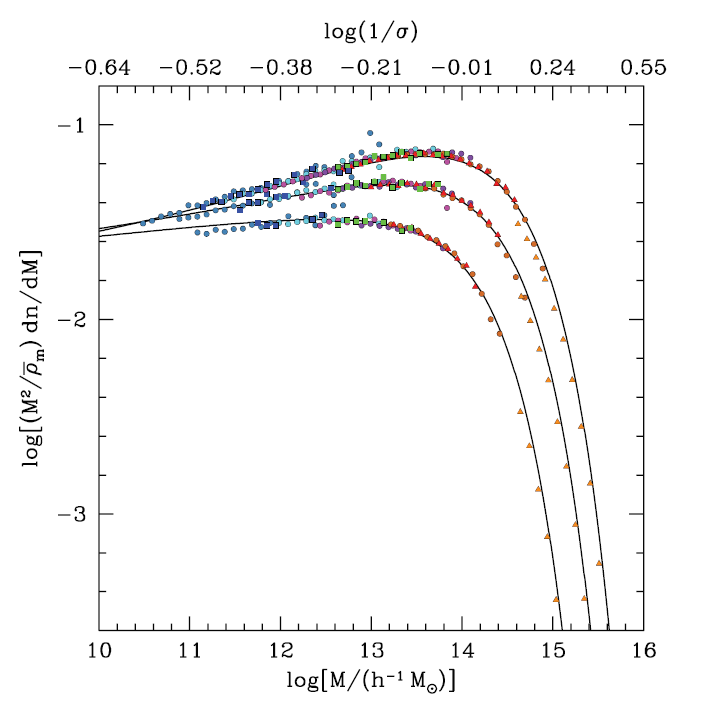
\includegraphics[width=0.9\textwidth]{images/halo_mass_function.png}
    \caption{Halo mass function for three different overdensities, $\Delta = 200, 800, 3200$ from top to bottom (points). The different points represent the different simulations used. The solid black lines are best fits for each value of the overdensity $\Delta$. They are all three Schechter functions, with varying multiplicity functions to get the best fit to their respective data points. Credit \textcite{Tinker2008}.}
    \label{halo_mass}
\end{figure}

\subsubsection{Galaxies}
Dark matter halos formed before baryonic matter could gather in densities even close to that needed to form stars, as there is 6-7 times more dark matter than baryonic matter. The dark matter halos created a gravitational potential well which gave room for the primordial baryonic matter (ionized hydrogen gas) to start collapsing. 

As the density of the gas increases, temperature increases and halts the collapse, but through several radiation cooling processes the gas is able to collapse enough for fusion to start and stars to be born. Because of the halos role as initial potential wells, the baryonic matter collapses in such a way that the angular momentum of its initial components get transferred to the galaxy as a whole, and the result is a rotating disk galaxy at the center of the halo. This is the birth process of galaxies.

Galaxies are mainly composed of stars and hot gas, with a smaller contribution of stellar remnants, cold gas and dust. Hot gas is hydrogen gas that is fully ionized and does not collapse into stars, while cold gas has a much lower temperature and can contribute to star formation. There are at least two trillion galaxies in the observable Universe \parencite{Conselice2016}, with stellar masses ranging from less than $10^6 M_{\odot}$ to $10^{12} M_{\odot}$ and larger. 

It has been found that a large fraction of galaxies are gravitationally bound to each other in groups and clusters.
Galaxy clusters are the largest gravitationally bound systems in the Universe, and can span a distance of several megaparsecs. They typically contain more than a hundred galaxies, as well as large amounts of intergalactic gas. Galaxies in clusters serve an important purpose to astrophysicists, as they essentially function as tracers of the largest halos in the Universe.

As galaxies reside in the center of halos, they too follow a hierarchical growth pattern where larger galaxies are created through the merger of smaller galaxies. All galaxies start of as disk galaxies, so galaxies that have an elliptical component of stars and gas with pressure dominated random motions and which extends in all directions from the center, are results of the merging of galaxies. In galaxy clusters the density of galaxies is much higher than the average of the Universe, so the likelihood of a galaxy merger is higher there. Therefore clusters contain a higher percentage of elliptical galaxies.

A very important property of the galaxy population is the galaxy luminosity function, which gives the number density of galaxies as a function of their luminosity. The luminosity of a galaxy is directly proportional to its stellar mass, so the luminosity function also gives us the mass distribution of galaxies. Mathematically, the luminosity function is defined as $\phi(L)dL$, where $\phi(L)dL$ is the number density of galaxies in the luminosity range $L \pm dL/2$. In 1976 Paul Schechter proposed a fit to the luminosity function of galaxies on the form

\begin{equation} \label{lum_func}
    \phi(L)dL = \phi^*(L/L^*)^{\alpha}\exp{(-L/L^*)}dL/L^*,
\end{equation}

where $\phi^*$ is a normalization, $L^*$ is the characteristic luminosity for that sample of galaxies (it will differ for instance for galaxies within a cluster compared to isolated galaxies) and $\alpha$ is the slope of the power law where $L<<L^*$ \parencite{Schechter1976}. Figure \ref{luminosity_function} shows the luminosity function (points) as well as the best fit for equation \ref{lum_func} (solid line). This Schechter function is still a good fit to this day, and is in excellent agreement for galaxies with $L>>L^*$. For the low mass range of galaxies, the parameter $\alpha$ must be found, and this is one of the challenges of astrophysicists that study galaxy properties.

\begin{figure}
    \centering
    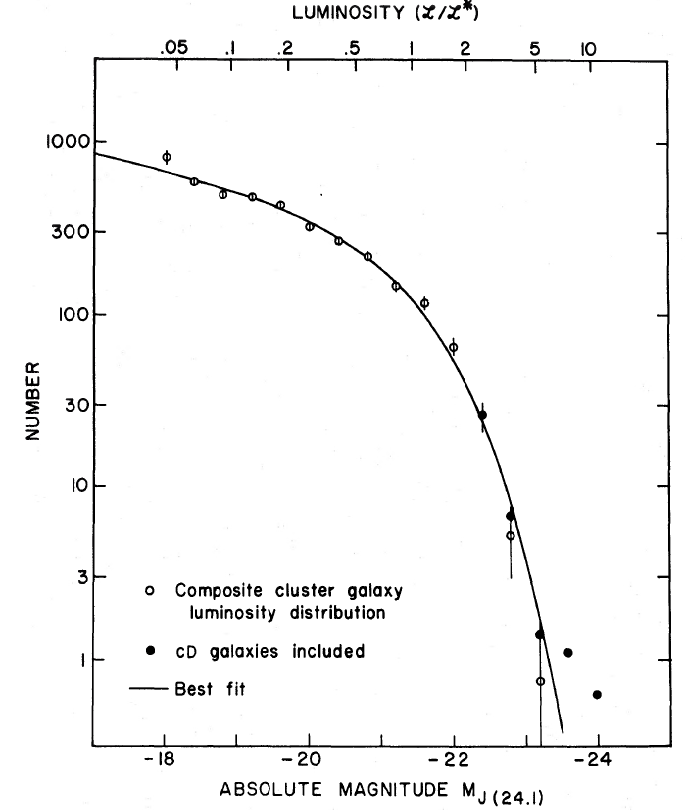
\includegraphics[width=0.9\textwidth]{images/luminosity_function.png}
    \caption{The luminosity function at redshift 0. The open circles correspond to observed galaxies in clusters, while the filled in circles denote cD galaxies (giant ellipticals). The solid line shows the best fit using equation \ref{lum_func}. Credit: \textcite{Schechter1976}.}
    \label{luminosity_function}
\end{figure}

\subsubsection{The Stellar-to-Halo mass relation}

The Stellar-to-Halo mass relation (hereafter, SHM relation) gives the stellar mass of a galaxy as a function of its host halo mass. This is particularly difficult to determine empirically, as it is not possible to directly measure the dark matter halo mass.

One way of looking for this relation is through a method called abundance matching. In abundance matching, the numerically found halo mass function and the observationally found luminosity function are combined. This is done using the simple assumption that the largest halo contains the largest galaxy, the second largest halo contains the second largest halo and so on. By mapping each galaxy to its corresponding halo in such a fashion, the shape of the SHM relation can be found directly.

Using abundance matching, the SHM relation has been found to be well described by a double power law with different slopes for the low-mass and high-mass end of the spectrum \parencite{Behroozi2013}. 

Other ways of studying the SHM relation could be through simulations which include halo and stellar mass like IllustrisTNG, or inferring the halo mass empirically by using the rotational curves of disk galaxies (see Section \ref{lates}), gravitational lensing and other mobservational methods.

\subsection{Galaxy evolution and classification}

As soon as telescopes became good enough to clearly make out galaxies in the sky, it became apparent to astronomers that galaxies come in many different shapes and sizes. The morphology of the galaxy is closely linked to other properties of the galaxy and is therefore important for the classification of galaxies. Edwin Hubble classified galaxies on a spectra \parencite{Hubble1926}, with elliptical galaxies (galaxies that have a dominant spheroidal component) on one end of the spectrum and spiral galaxies (galaxies with a prominent disk component) on the other (Figure \ref{hubble}). The galaxy types were presented as a sequence, so Hubble deemed it convenient to use the adjectives ``early'' and ``late'' to describe the two extreme ends of the spectrum. He did consider the fact that these words might be confusing because of their temporal connotations, but went ahead with using ``early'' and ``late'' as a proxy for ``less complex'' and ``more complex'', respectively. Indeed this turned out to be confusing, as it is now established that galaxies actually evolve with time along the sequence, starting out as late type disk galaxies and often ending up as more massive early type ellipticals.

\begin{figure}
    \centering
    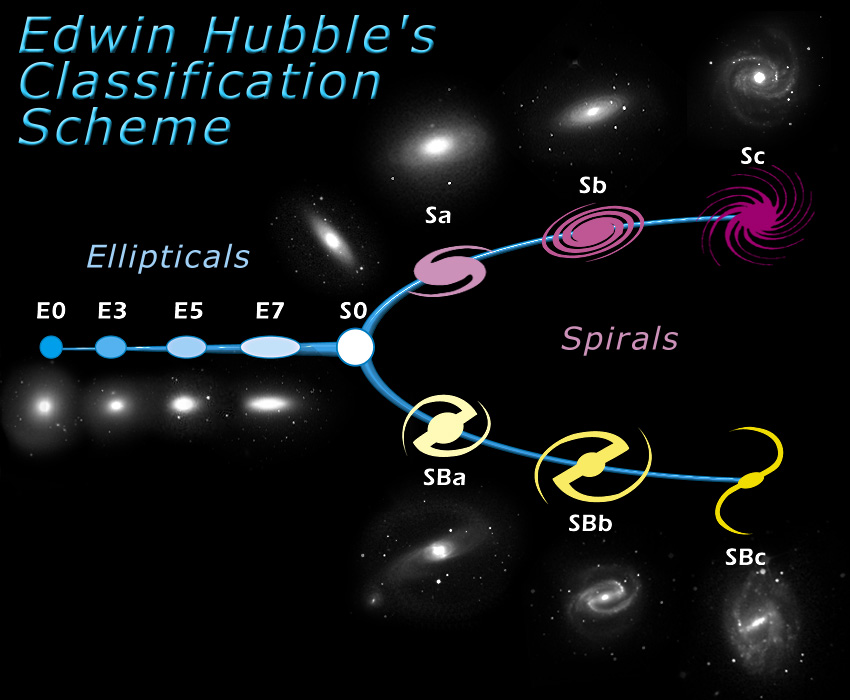
\includegraphics[width=0.7\textwidth]{images/hubble.jpg}
    \caption{Chart from 1999 showing the original classifications of galaxy morphology. Credit: ESA/Hubble}
    \label{hubble}
\end{figure}

In the $\Lambda$CDM model, galaxies grow through mergers. Mergers are separated into two types, major and minor mergers. Major mergers are events where two galaxies of equal size collide and become one galaxy, while minor mergers happen when one of the galaxies is significantly smaller than the other. Simulations have shown that a major merger between two disk galaxies produces an elliptical. The Milky Way, which is a large ($M_*>10^{10} M_\odot$) spiral galaxy has probably grown through many smaller minor mergers, and thus kept its disky shape.

It is not always easy to distinguish between a disky elliptical and a spiral with a large spheroidal component (bulge). Some galaxies are also in the middle of a merging process. These can have very irregular shapes, and so are hard to classify. Other galaxies are very small, so called dwarf galaxies. These galaxies tend to have very little stellar mass compared to dark matter, so they do not exhibit the properties of ellipticals, even though they may be more elliptical in shape.

Galaxies were initially seperated into the two types (early and late) by their shape, but as astronomers have studied these different galaxy categories, it has become apparent that there are many other properties that also serve to distinguish the two types. Table \ref{morphologies} gives a quick overview of the main properties of early and late type galaxies, while the rest of this Section explains them in more detail.


\begin{table}
\begin{center}
\caption{Galaxy properties by morphology type.}
\label{morphologies}
\begin{tabular} { l| c c } 
 \hline
 \hline
  & Early type & Late type \\
 \hline
 Shape & Spheroidal & Disk \\
 Color & Red & Blue \\
 Velocity direction& Radial & Circular \\
 Stellar population & Older & Younger \\
 Star formation rate & Low & High \\
 Size & Smaller & Larger \\
 Gas and dust & Little & More \\
  
 \hline 
\end{tabular}
\end{center}
\end{table}

\subsubsection{Elliptical (early type) galaxies}
Elliptical galaxies are mainly pressure-dominated systems, meaning that the motion of the stars is predominantly radial. The largest galaxies in the Universe tend to be ellipticals, but they come in all sizes. The star population of ellipticals is generally older than that of spirals, and there is usually little to no star formation. There is very little gas and dust in ellipticals, and they tend to emit more light in the redder end of the electromagnetic spectrum. Early type galaxies are less common than late type galaxies, and are more usually found in galaxy clusters.

\subsubsection{Spiral (late type) galaxies} \label{lates}
Late type galaxies have a prominent disky component which orbits around the galaxy's center. The rotational velocity of the disk is typically larger than the velocity dispersion of the galaxy's bulge. The stars in a spiral galaxy are usually younger than those in early types. There is a lot of gas and dust present in spirals, giving rise to ongoing star formation. Late type galaxies are bluer in color than early types. Field galaxies, which are not part of any galaxy cluster, are predominantly spirals. 


The rotational velocities of the stars at different radii in the disk of spiral galaxies can be measured observationally, and plotting the velocity as a function of radius gives us the velocity curve of the galaxy. If the mass in the galaxy was solely made up of the gas and stars that we are able to detect optically, we would expect the velocity curve to drop off as we get to the outer parts of the galaxy. Assuming the particles move in circular orbits around the center of mass, the circular velocity at a given radius is given by the formula

\begin{equation}
    v_{circ} = \sqrt{GM(<R)/R}, 
\end{equation}

where $M(<R)$ is the total mass within radius $R$. However, the observational data shows that the velocity curve does not fall off towards the outer parts of the galaxy, but actually flattens out. An example of this can be seen in Figure \ref{rotation_curves}. There the rotation curves of several spiral galaxies are shown, along with the curve showing the expected fall off of velocity if there was no dark matter (long-dashed line). This perplexed early astrophysicists, as the mass inside the outer radius must be much greater than that which could be accounted for by the stars and gas in the galaxy. An effort to solve this problem led to the theory of dark matter, and later to the $\Lambda$CDM model.

\begin{figure}
    \centering
    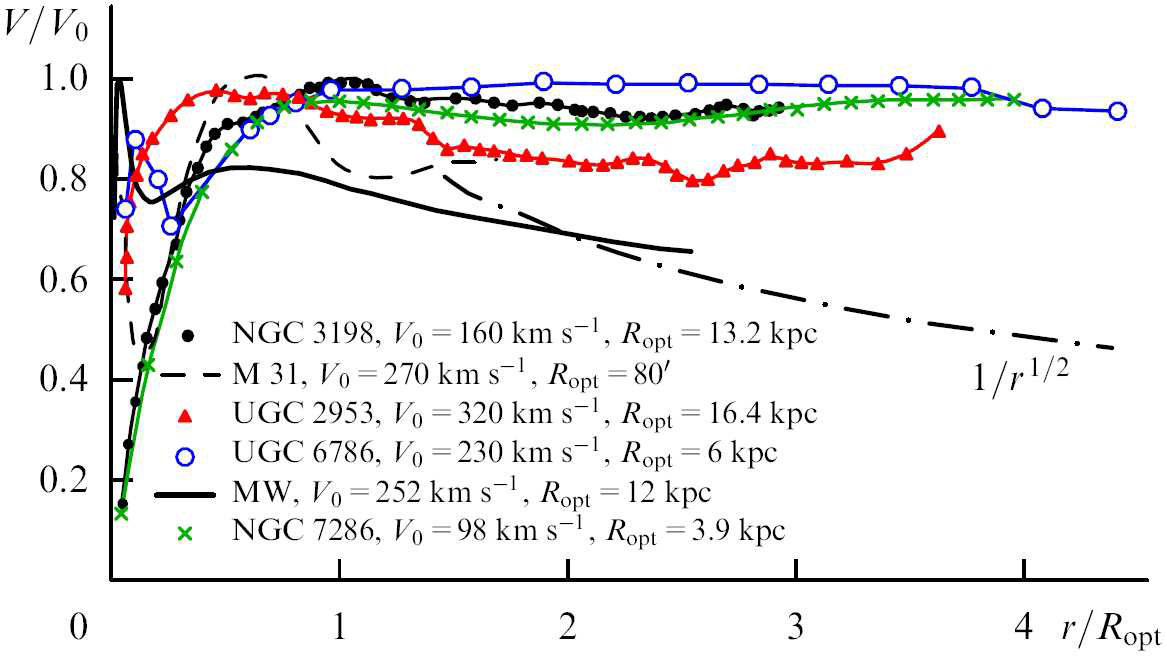
\includegraphics[width=0.9\textwidth]{images/rotation_curves.png}
    \caption{Rotation curves for several spiral galaxies (points). The velocities are normalized with respect to each of the galaxies maximum velocity. Radial distances are in units of the optical radius $R_{opt}$ (the radius within 83\% of the light is enclosed). The long-dashed line shows the expected Keplerian curve if there was no dark matter. Credit: \textcite{Zasov2017}.}
    \label{rotation_curves}
\end{figure}

\subsubsection{Classifying galaxies}

An important factor in many studies of galaxy formation and evolution is looking at and comparing the properties of the two main morphological types of galaxies. In observations, a visual classification method is usually used, although it is intensively time-consuming. %you can cite here galaxy zoo (https://www.zooniverse.org/projects/zookeeper/galaxy-zoo/) 
Other methods have therefore been devised for identifying early and late-type galaxies in simulations. In many studies, several classification methods are used in conjunction. 

As early-type galaxies have much less cold gas than late-type galaxies, a simple division in the galaxy population based on the gas fraction (gas mass divided by stellar mass) will be effective at roughly separating the two types. Gas is not distributed evenly in galaxies however, so it is important to consider the physical volume where the gas fraction is calculated. A large volume will inevitably contain more hot (not star-forming) gas and potentially allow for early-type galaxies to be considered as late types. Late-type galaxies also have a wide range of gas fractions. The most massive spiral galaxies ($M_\ast \sim 10^{11} M_\odot$) can contain as little as 5\% gas, while low-mass disks ($M_\ast < 10^{9.5} M_\odot$) can contain up to 80\% \parencite{Mo2010}. In \textcite{Ferrero2020} gas fraction was used as one of two criteria of morphological classification. Galaxies with a gas fraction of less than 0.1 were considered for early types, while those with more were potential candidates for late-type classifications.

Another way of separating galaxies into the early and late-type categories is by using the specific star formation rate (sSFR). The sSFR of a galaxy is the galaxy's star formation rate divided by the stellar mass content of the galaxy. As an example, a galaxy with a stellar mass of $10^{10} M_\odot$ that produces stars with a total mass $1 M_\odot$ has a sSFR of $10^{-10}$, commonly expressed as $\log(sSFR) = -10$. Galaxies are tagged as ``quenched'' or ``main-sequence'', where quenched galaxies have little to no star formation, while main-sequence galaxies have a significant amount of star formation \parencite{Noeske2007}. More formally, they are separated by how far from the ridge of the star-formation main-sequence they are found. In a study using the data from the TNG simulation, \textcite{Genel2017} defined the ridge of the main-sequence as the mean of the sSFR for galaxies with mass $10^{9} M_{\odot} < M_* < 10^{10.5} M_{\odot}$, and takes a value of $\log (sSFR[Gyr^{-1}]) = -0.94$ for $z=0$. Galaxies are then considered `main-sequence' if their sSFR are within 0.5 dex of this value. A simpler criteria for main-sequence galaxies is to drop the upper bound and include all galaxies that have sSFR more than 0.5 below the ridge. ``Quenched'' galaxies are defined as those with sSFR at least 1 dex below the ridge. 

A common way of estimating a galaxy's ``diskyness'' is to use the rotational ($K_{rot}$) to total ($K$) kinetic energy parameter $\kappa_{rot}$. 
\begin{equation}
    \kappa_{rot} = \frac{K_{rot}}{K} = \frac{\sum_{i=1}^{N} m_i (j_{z, i}/R_i)^2}{\sum_{i=1}^{N} m_i v_i^2},
\end{equation}
where $j_{z, i}$ is the z-component of the specific angular momentum ($\vec{j} = \vec{r} \times \vec{v}$), $m_i$ is the mass, and $R_i$ is the projected radius of stellar particle $i$ in the xy-plane. 
This value indicates how much of the kinetic energy of the galaxy is invested in the ordered rotation about its axis. To calculate $\kappa_{rot}$, the axis of rotation must first be found. The galaxy is then rotated such that the z-axis of the galaxy's coordinate system is pointed in the direction of the axis of rotation, and $\kappa_{rot}$ is calculated.
For a perfect disk galaxy that is totally rotationally supported $\kappa_{rot} = 1$, while for a totally pressure supported system, $\kappa_{rot}$ would approach zero. In \textcite{Sales2012}, galaxies were classified as early type if they had $\kappa_{rot} < 0.5$ and late type for $\kappa_{rot} > 0.7$. This leads to a significant amount of ``intermediate types'', but other works have simply made use of a single cut at $\kappa_{rot} = 0.6$ \parencite{Ferrero2020}. Figure \ref{kappa_rot} shows the face-on and edge on structure of three rotated galaxies with varying values of $\kappa_{rot}$. The higher the rotational to kinetic energy ratio, the more disk shaped is the galaxy.


\begin{figure}
    \centering
    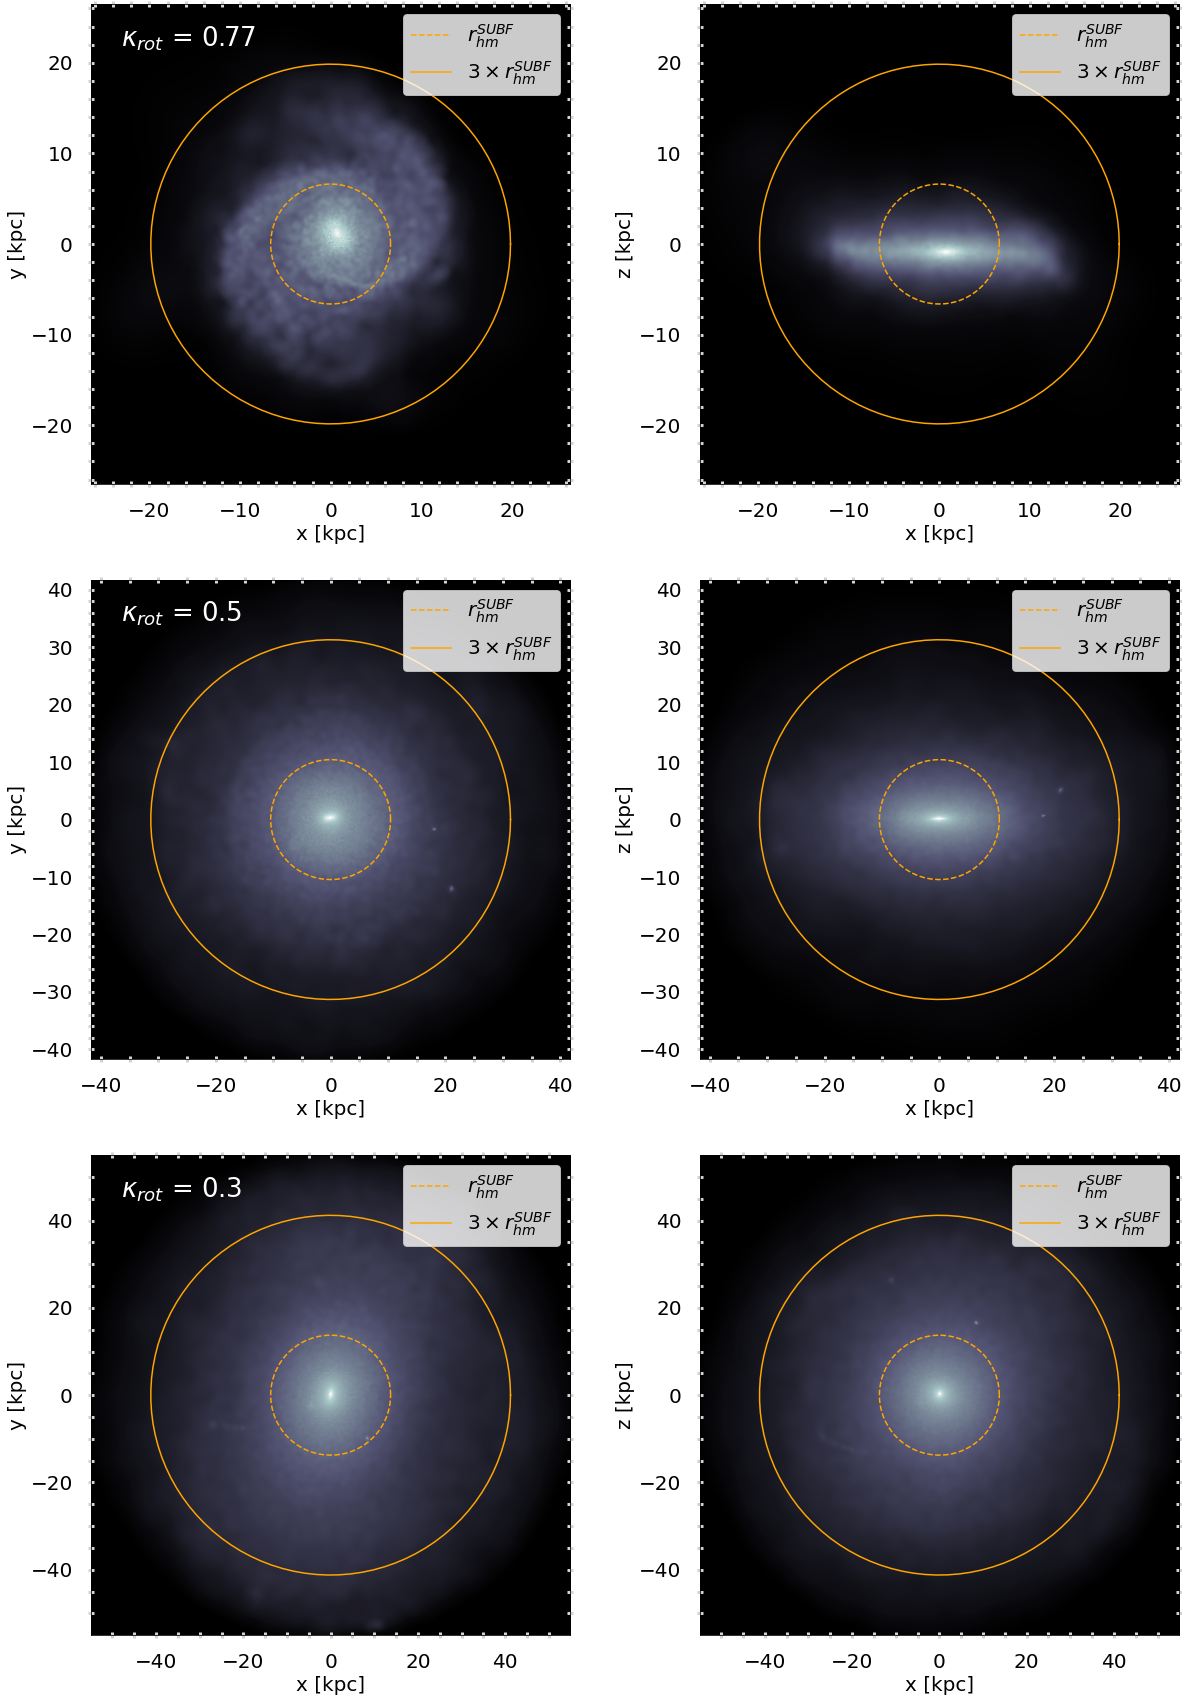
\includegraphics[width=0.85\textwidth]{images/kappa_rot.png}
    \caption{The stellar mass density projections of three different galaxies with $\kappa_{rot} =$ 0.77, 0.5 and 0.3, from top to bottom. The galaxies are shown both face on (right) and edge on (left).}
    \label{kappa_rot}
\end{figure}

\subsection{Galaxy properties}
In this report I will be looking at many of the main galaxy properties that have been explored throughout the years. We will only be looking at the relations in the present time, $z=0$, but the relations have been studied across redshifts and many are redshift-dependent.

\subsubsection{The Tully-Fisher relation}

\textcite{TullyFisher1977} found a surprisingly good correlation between the luminosity of a spiral galaxy and the characteristic rotational speed of its disk on the form of a simple power law with index $\alpha$,

\begin{equation}
    L \propto V_{rot}^\alpha.
\end{equation}

This is known as the Tully-Fisher relation (TFR) (Figure \ref{tully_fisher}). As stellar mass is directly proportional to the luminosity, this gives us the ability to estimate stellar mass from a simple measurement of the rotational velocity.

\begin{equation}
    M_* \propto V_{rot}^\alpha 
\end{equation}

$\alpha$ was found to be 3.7 \parencite{TullyFisher1977}. Later work has found $\alpha$ to lie between 3 and 4 \parencite{Lelli2019, Bloom2017}.

This relation is a great tool for estimating the distance to a galaxy, as the predicted total luminosity can be compared to the apparent magnitude at Earth. For numerical simulations, being able to reproduce the TFR is an essential way to check if the model is reliable.

\begin{figure}
    \centering
    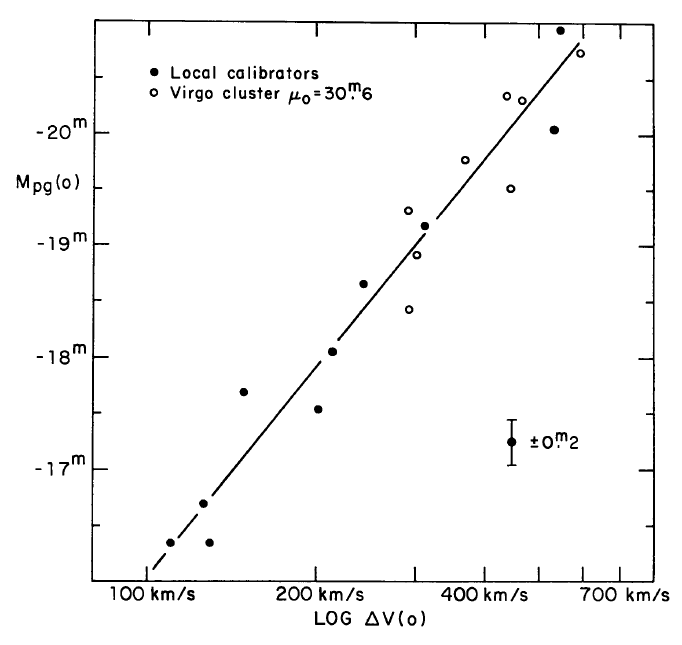
\includegraphics[width=0.9\textwidth]{images/tully_fisher.png}
    \caption{The original figure from the 1977 paper by R.B. Tully and J.R. Fisher, showing the linear fit for the luminosity - velocity values in the log-log plane. Credit: \textcite{TullyFisher1977}}
    \label{tully_fisher}
\end{figure}

\subsubsection{The Faber-Jackson relation and the Fundamental Plane}
At around the same time \textcite{TullyFisher1977} linked the velocity dispersion and luminosity of early type galaxies. In observations, the only velocities of the components of a galaxy we can measure are the line-of-sight velocities ($V$). These are calculated using the observed Doppler shift in the galactic spectrum. The velocity dispersion of a galaxy is then defined as the standard deviation of the line-of sight velocities.

\begin{equation} \label{standard_dev}
    \sigma^{2} = \frac{1}{N} \sum_{n=1}^{N} (V_{i} - \overline{V})^2
\end{equation}

The proposed relation between $\sigma$ and $L$ was on the form of a power law as well,

\begin{equation}
    L \propto \sigma^{\gamma},
\end{equation}

with a power law index $\gamma$ of approximately 4 (Figure \ref{faber_jackson}).

\begin{figure}
    \centering
    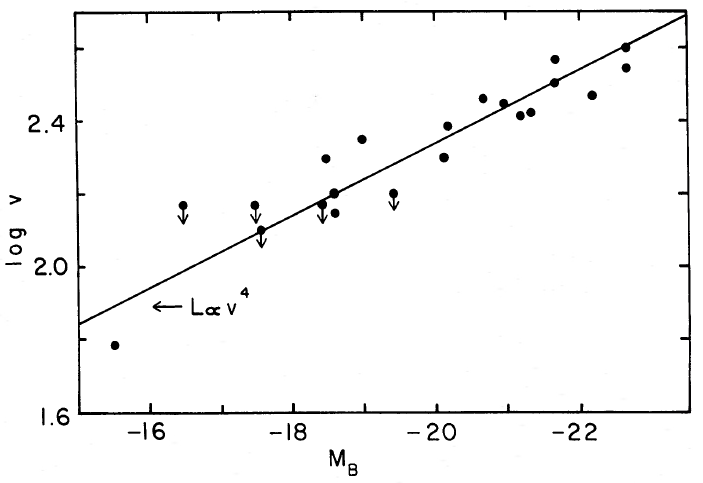
\includegraphics[width=0.9\textwidth]{images/faber_jackson.png}
    \caption{The original fit for the Faber-Jackson relation as presented in the 1976 paper. It shows the velocity dispersion as function of the luminosity in the log-log plane (dots), along with a power law with index 4 (solid black line). Credit: \parencite{TullyFisher1977}}
    \label{faber_jackson}
\end{figure}

This is known as the Faber-Jackson (FJ) relation. The scatter in the FJ relation was larger than that found for the TFR however, and it was later found that the velocity dispersion was dependent on the size of the galaxy. This dependency also took the form of a power law, and so the velocity dispersion is more accurately described by the function

\begin{equation}
    \sigma \propto L^a R^b.
\end{equation}

With the radius added into the equation, the scatter became much less significant. Most ellipticals are found on the same plane in ${\sigma, R, L}$ space. This became known as the Fundamental Plane (FP) \parencite{Djorgovski1987}, and is also something which successful numerical simulations must reproduce.

\subsubsection{Color bimodality}
Color, in astrophysics, is defined as the difference in magnitudes measured for a galaxy by two different optical filters. A galaxy that is "blue" has a larger amount of blue light than red. In general, galaxies are found to inhabit one of two groups on a color-mass diagram, blue or red (see Figure \ref{color_bimodality}). The blue galaxies are most often late type galaxies, while the red ones are mainly early types. There are many factors that contribute to the color of a galaxy, like stellar age and metallicity as well as the amount of gas the light has passed through and its metallicity.

\begin{figure}
    \centering
    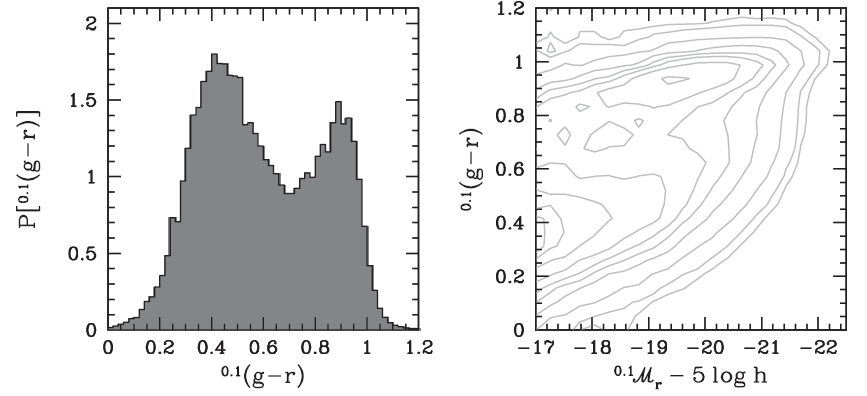
\includegraphics[width=0.9\textwidth]{images/color_bimodality.png}
    \caption{To the left: The probability density of the g-i color for over 350 000 galaxies in the Sloan Digital Sky Survey. To the right: The color-magnitude contour map for the same galaxies, clearly showing two distinct populations. Credit: \textcite{Mo2010}}.
    \label{color_bimodality}
\end{figure}



\section{Method} \label{method}
\subsection{IllustrisTNG}
IllustrisTNG \footnote{https://www.tng-project.org/} is the follow-up project after the success of the Illustris simulations \parencite{Springel2017, Pillepich2017,Naiman2018, Nelson2017, Marinacci2018}. It is a huge project, built upon a magneto-hydrodynamical cosmological simulation code with added physical processes on a subgrid level \parencite{Weinberger2016}. Adding physical processes like gas radiation, star formation, stellar feedback through supernova explosions, supermassive black hole accretion and magnetic fields is essential to model galaxy formation and evolution and allows for a much better comparison to reality compared to dark matter-only simulations. The data output from the simulations is extensive, and is not meant to be analyzed all in one go, but rather through a series of analyzes, each targeting a specific scientific question. 


\subsubsection{The simulations}
The IllustrisTNG project includes 18 different simulations with varying resolutions, spatial size, and included physics. There are three main simulations, TNG300, TNG100, and TNG50, that differ in volume and resolution. The details of these are summed up in Table \ref{TNG}. Each of the main simulations has been run at three different resolution levels, which makes it possible to study how the outcome is affected by changing only the resolution in a given simulation. TNG100 has a physical box volume of $110.7^3 \, $Mpc$^3$, and a baryonic particle resolution of $1.4 \times 10^6 M_{\odot}$, while the TNG300 simulation has a volume of $302.6^3 \, $Mpc$^3$ and a baryonic particle resolution of $1.1 \times 10^7 M_{\odot}$. The newly released third simulation, TNG50, has a smaller volume of $51.7^3 \, $Mpc$^3$, but with a much higher baryonic particle resolution of $8.5 \times 10^4 M_{\odot}$. 

In this project, a large statistical sample of galaxies was needed, as well as a resolved structure of the inner part of the galaxies to calculate the different properties, so the TNG100 simulation was the best choice with respect to size and resolution. The TNG100-1 simulation data, which is the highest available resolution for TNG100, has been used throughout the project and will from now on be referred to as TNG only. A visual representation of parts of the simulations can be seen in Figure \ref{tng_illustration}. For its cosmology parameters TNG uses the results from the Planck Collaboration, which are given by $\Omega_{\Lambda,0} = 0.6911$, $\Omega_{m,0}=0.3089$, $\Omega_{b,0}=0.0486$, $\sigma_8=0.8159$, $n_s=0.9667$ and $h = 0.6774$ \parencite{Planck2016}.

\begin{figure}
    \centering
    \includegraphics[width=0.9\textwidth]{images/TNG.png}
    \caption{A composite image that illustrates the two simulations TNG100 and TNG300. In the background is the dark matter distribution for the whole TNG300 volume. In the upper right is the stellar mass distribution across the entire TNG100 volume. The panels on the left show galaxy-galaxy interactions, while the panels on the right show the stellar light projections of two $z=0$ galaxies. Credit: TNG Collaboration}.
    \label{tng_illustration}
\end{figure}

\begin{table}
\begin{center}
\caption{The simulation details for the three main TNG simulations. $N_{DM}$ is the amount of dark matter particles. $m_{DM}$ and $m_{baryon}$ is the mass of the dark matter and baryonic particles, respectively.}
 \label{TNG}
\begin{tabular}{ l| c c c c c } 
 \hline
 \hline
   &  Volume [$Mpc^3$] & $N_{DM}$ & $m_{DM}$ [$M_{\odot}$] & $m_{baryon}$ [$M_{\odot}$] \\
 \hline
 TNG50 & $51.7^3$ & $2163^3$ & $4.5 \times 10^5 $ & $8.5 \times 10^4 $ \\ 
 TNG100 & $110.7^3$ & $1820^3$ & $7.5 \times 10^6 $ & $1.4 \times 10^6 $  \\ 
 TNG300 & $302.6^3$ & $2500^3$ & $5.9 \times 10^7 $ & $1.1 \times 10^7 $  \\ 
 \hline 
 \end{tabular}
\end{center}
\end{table}

\subsubsection{Data products}
All the Illustris-TNG data is publically available online at the TNG webpage\footnote{https://www.tng-project.org/data/}. The data products that are available for each simulation are snapshots, group catalogs, and merger trees as well as some supplementary data sets. There are five different particle types in the simulations, and each has its properties stored as particle fields. These fields include information like position, kinematic data, and chemical composition. For each different run of the simulation, 100 snapshots are created, which are taken at specific redshifts. They include all the particles in the whole volume of the simulation, with 20 of them including all the fields for each particle as well.

The group catalogs provide a convenient way to quickly access already calculated properties of the different halos and subhalos instead of dealing with all the particles in a snapshot. This saves a lot of time and effort but gives the user less control over what can be analyzed. There is one group catalog for each snapshot, and this includes two types of objects, Friends-of-Friends (FoF) and SUBFIND. The FoF catalog contains all the halos, and the SUBFIND catalog contains all the subhalos and their associated galaxy (if there is any) for each halo. Each subhalo has a parent halo, and the largest subhalo in each halo is the central subhalo. The merger trees data products contain the merger history of each subhalo.

This project makes use of the group catalogs and particles for the $z = 0$ snapshot.

\subsubsection{Sample reduction}

The TNG documentation recommends filtering out all subhalos that are flagged with the $SubhaloFlag$ field, and so these were cut from the data. They are most probably subhalos of non-cosmological origin, and so should not be considered real galaxies.

For this project, only the central galaxies in each halo are selected. The FoF catalog contains the index for the largest subhalo in each halo, so combining this information with the SUBFIND catalog allows one to create a subset of the data that contains only the central galaxies.

Only galaxies with stellar mass greater than $10^{9.5} M_{\odot}$ are used, which corresponds to about 4500 stellar particles.

\subsection{Galaxy sizes}
When observing galaxies with telescopes, there is always the problem of contamination of the measurements by surrounding sources as well as background radiation. As such, when the images are processed, aperture sizes have to be chosen with care for each identified galaxy. A larger aperture will be sure to contain most of the light from the galaxy but might overshoot by including surrounding light as well. However, choosing a too small aperture will result in lost data, and as such a smaller apparent galaxy. Usually a circular or elliptical aperture with a calculated radius to balance these two issues is chosen.

In simulations, we are not limited by hardware, attenuation, and background light. A cut-off point still needs to be determined. SUBFIND does this for the dark matter part of the simulation, separating out subhalos from larger halos. The galaxy properties of that subhalo are then calculated using all the stellar and gas particles in the subhalo and saved in the group catalog. 


When comparing simulation data to observational data, there are many ways to emulate the finite size of observed galaxies. Calculating luminosities and selecting a cut-off point at the faint end, using a spherical volume with a radius that is a multiple of their particular effective radius, or a fraction of the virial radius of the parent subhalo are some of the most commonly employed methods. For this work, the galaxy size is chosen to be a spherical volume with a radius ($R_{gal}$) equal to 15 \% of the subhalo's virial radius.

\subsection{Galaxy properties}

\subsubsection{Magnitude and colors}

The absolute magnitude ($\mathcal{M}$) is a measure of the total luminosity ($L$) of the galaxy such that $\mathcal{M} = -2.5 \log(L/L_\odot) + \mathcal{M}_\odot$, where $L_\odot$ is the solar luminosity and $\mathcal{M}_\odot$ is the solar magnitude.

For the SUBHALO group catalog, the \texttt{SubhaloStellarPhotometrics} field gives the magnitudes based on the summed up luminosities of all the stellar particles in the Subhalo. Our luminosities are determined by summing the luminosities within $R_{gal}$. Eight bands are available, but here only the g- and i-band are used. 

The g-i colors are calculated by simply subtracting the i-band magnitude from the g-band magnitude.

\subsubsection{Masses}

In SUBFIND, masses for each particle type are calculated by summing up all the masses of that particle type belonging to the halo. Values for the mass within the half-mass radius, two times the half-mass radius and the radius at which the maximum rotational velocity is found are also available.

The stellar masses of the galaxies studied using the particles are the summed up masses of all stellar particles within $R_{gal}$.

\subsubsection{Size}
For the group catalog, the \texttt{SubhaloHalfmassRadStellar} field has been used as the effective radius. The half-mass radius is the radius of a spherical volume within which half the stellar mass is found. It is the 3D half-mass radius ($R_e$), as it is not a projected quantity.

The half-mass radii of the galaxies calculated using the particles are calculated using the same method, but with the total stellar mass calculated within $R_{gal}$.

\subsubsection{Velocities}

Galaxy velocities are usually given by the velocity dispersion and rotational velocity for early and late-type galaxies, respectively. This is because of the difference in the shape of the two galaxy types. It makes more sense to talk about velocity dispersion in a spheroidal pressure-dominated system and rotational velocity in a rotating disk.

In SUBFIND, the field \texttt{SubhaloVMax} gives the maximum value for the spherically averaged rotation curve of a given galaxy. As the rotational curves are nearly flat for large enough radii, it should not be very important at which specific radius the observational rotational velocity is measured, as long as it is in the flat part of the curve. For observational data, a common practice is to look at the rotational velocities of stars in the outer part of the galaxy. To compare with SUBFIND's \texttt{SubhaloVMax}, the rotational velocity at a radius of $2.2 \times R_e$ was calculated for all galaxies.


In observations, the only velocities of the components of a galaxy we can measure are the line-of-sight velocities. These are calculated using the observed Doppler shift in the galactic spectrum. The velocity dispersion of a galaxy is then defined as the standard deviation of the line-of sight velocities.

\begin{equation} \label{standard_dev}
    \sigma^{2} = \frac{1}{N} \sum_{n=1}^{N} (V_{i} - \overline{V})^2
\end{equation}

If the velocity dispersion tends to fall off at larger radii, and the galaxy has an ellipsoid shape, the angle at which the galaxy is viewed will affect the observed velocity dispersion. To compensate for this when comparing simulations to observations, velocity dispersions in simulations may be calculated in three different projections of the galaxy and averaged over these. 

\begin{equation} \label{sigma1}
    \sigma^{2} = \frac{1}{3}(\sigma_x^2 + \sigma_y^2 + \sigma_z^2)
\end{equation}

In this work the velocity dispersion was calculated within the projected half-mass radius in each projection.

In SUBFIND, the velocity dispersion is simply calculated as the velocity dispersion of all the particles over the entire subhalo.


\subsection{Galaxy morphology classifications}

An important factor in many studies of galaxy formation and evolution is looking at the properties of the two morphological types of galaxies. As a visual classification method is intensively time-consuming, other methods have been devised for identifying early and late-type galaxies in simulations. In many studies, several of these classification criteria are used in conjunction.

\subsubsection{Gas fraction}
As early-type galaxies have much less cold gas than late-type galaxies, a simple cut in the galaxy population based on the gas fraction will be effective at roughly separating the two types. TNG doesn't differentiate between cold and hot gas, so it is important to consider the physical volume where the gas fraction is calculated. A large volume will inevitably contain more hot gas and potentially allow for early-type galaxies to be considered as late types. Late-type galaxies also have a wide range of gas fractions. The most massive spiral galaxies can contain as little as 5\% gas, while low-mass disks can contain up to 80\% \parencite{Mo2010}. In \textcite{Ferrero2020} galaxies with less than 10\% gas were considered for early types, while those with more were potential candidates for late-type classifications.

\subsubsection{Star formation rate}
Another way of separating galaxies into the early and late-type categories is by using the specific star formation rate (sSFR). The sSFR of a galaxy is the galaxy's star formation rate divided by the stellar mass content of the galaxy. In this case, the galaxies are tagged as ``quenched'' or ``main-sequence'', where quenched galaxies have little to no star formation, while main-sequence galaxies have a significant amount of star formation. More formally, they are separated by how far from the ridge of the star-formation main-sequence they are found (//cite). In \textcite{Genel2017} the ridge of the main-sequence is defined as the mean of the sSFR for galaxies with mass $10^{9} M_{\odot} < M_* < 10^{10.5} M_{\odot}$, and takes a value of $\log (sSFR[Gyr^{-1}]) = -0.94$ for $z=0$. Galaxies are then considered `main-sequence' if their sSFR are within 0.5 dex of this value. ``Quenched'' galaxies are defined as those with sSFR at least 1 dex below the ridge.

\subsubsection{Rotational kinetic energy}
A common way of estimating a galaxy's ``diskyness'' is to use the rotational-to-total-kinetic-energy parameter $\kappa_{rot}$. 
\begin{equation}
    \kappa_{rot} = \frac{K_{rot}}{K} = \frac{\sum_{i=1}^{N} m_i (j_{z, i}/R_i)^2}{\sum_{i=1}^{N} m_i v_i^2},
\end{equation}
where $j_{z, i}$ is the z-component of the specific angular momentum ($\vec{j} = \vec{r} \times \vec{v}$), $m_i$ is the mass, and $R_i$ is the projected radius of stellar particle $i$ in the xy-plane. 
This value indicates how much of the kinetic energy of the galaxy is invested in the ordered rotation about its axis. To calculate $\kappa_{rot}$, the axis of rotation must first be found. The galaxy is then rotated such that the z-axis of the galaxy's coordinate system is pointed in the direction of the axis of rotation, and $\kappa_{rot}$ is calculated.
For a perfect disk galaxy that is totally rotationally supported $\kappa_{rot} = 1$, while for a totally pressure supported system, $\kappa_{rot}$ would approach zero. In \textcite{Sales2012}, galaxies were classified as early type if they had $\kappa_{rot} < 0.5$ and late type for $\kappa_{rot} > 0.7$. This leads to a significant amount of ``intermediate types'', but other works have simply made use of a single cut at $\kappa_{rot} = 0.6$.

\section{Results} \label{results}
In this section, the results of the analysis of the galaxy properties in TNG is presented, along with comparisons to observational data.

\subsection{Stellar-to-halo-mass relation}

The first relation that is studied is the stellar-to-halo-mass relation. It is one of the most fundamental relations that a hydrodynamical cosmological simulation should reproduce, as it ensures that we have the right distribution of halos and galaxies in our mock universe. This relation depends sensitively on the stellar mass content in the galaxy sample, and as such on the stellar mass definition used. The results for the fractional difference in stellar mass measurements for different definitions of galaxy radius are presented in Figure \ref{SM_fSM}. The most obvious result is the significant difference between $M^{SF}$ and $M_\ast^{2rhm}$, with the latter being at least 20 \% smaller for all stellar masses. $M_\ast^{15r200}$ and $M_\ast^{30kpc}$ are essentially indistinguishable from the SUBFIND values at masses below $10^{10.5} M_{\odot}$. For more massive galaxies there is an increasingly large difference between the two as well as compared to SUBFIND. At the higher mass end ($M^{SF}_\ast > 10^{11} M_{\odot}$), $M_\ast^{15r200}$ is about 10-15 \% smaller than SUBFIND, $M_\ast^{30kpc}$ is 12-40 \% smaller while $M_\ast^{2rhm}$ is approximately 30 \% smaller.


The reason that we get this difference in stellar mass using different apertures is of course that we are ``cutting off'' the continous stellar particle distribution in the halo. For large, diffuse galaxies, the effect will be most pronounced, and this is what we are indeed finding. A direct comparison of stellar masses found in galaxies between TNG and some other study would therefore be significantly affected by the choice of how stellar mass is defined. This is one of the reasons why galaxy properties are not directly comparable and we have to look at the trends in the properties rather than the exact values. However, this might also affect property relations, depending on how other properties are calculated. It is therefore interesting to see if other galaxy properties have a similar dependency on galaxy size definitions.

\begin{figure}
    \centering
    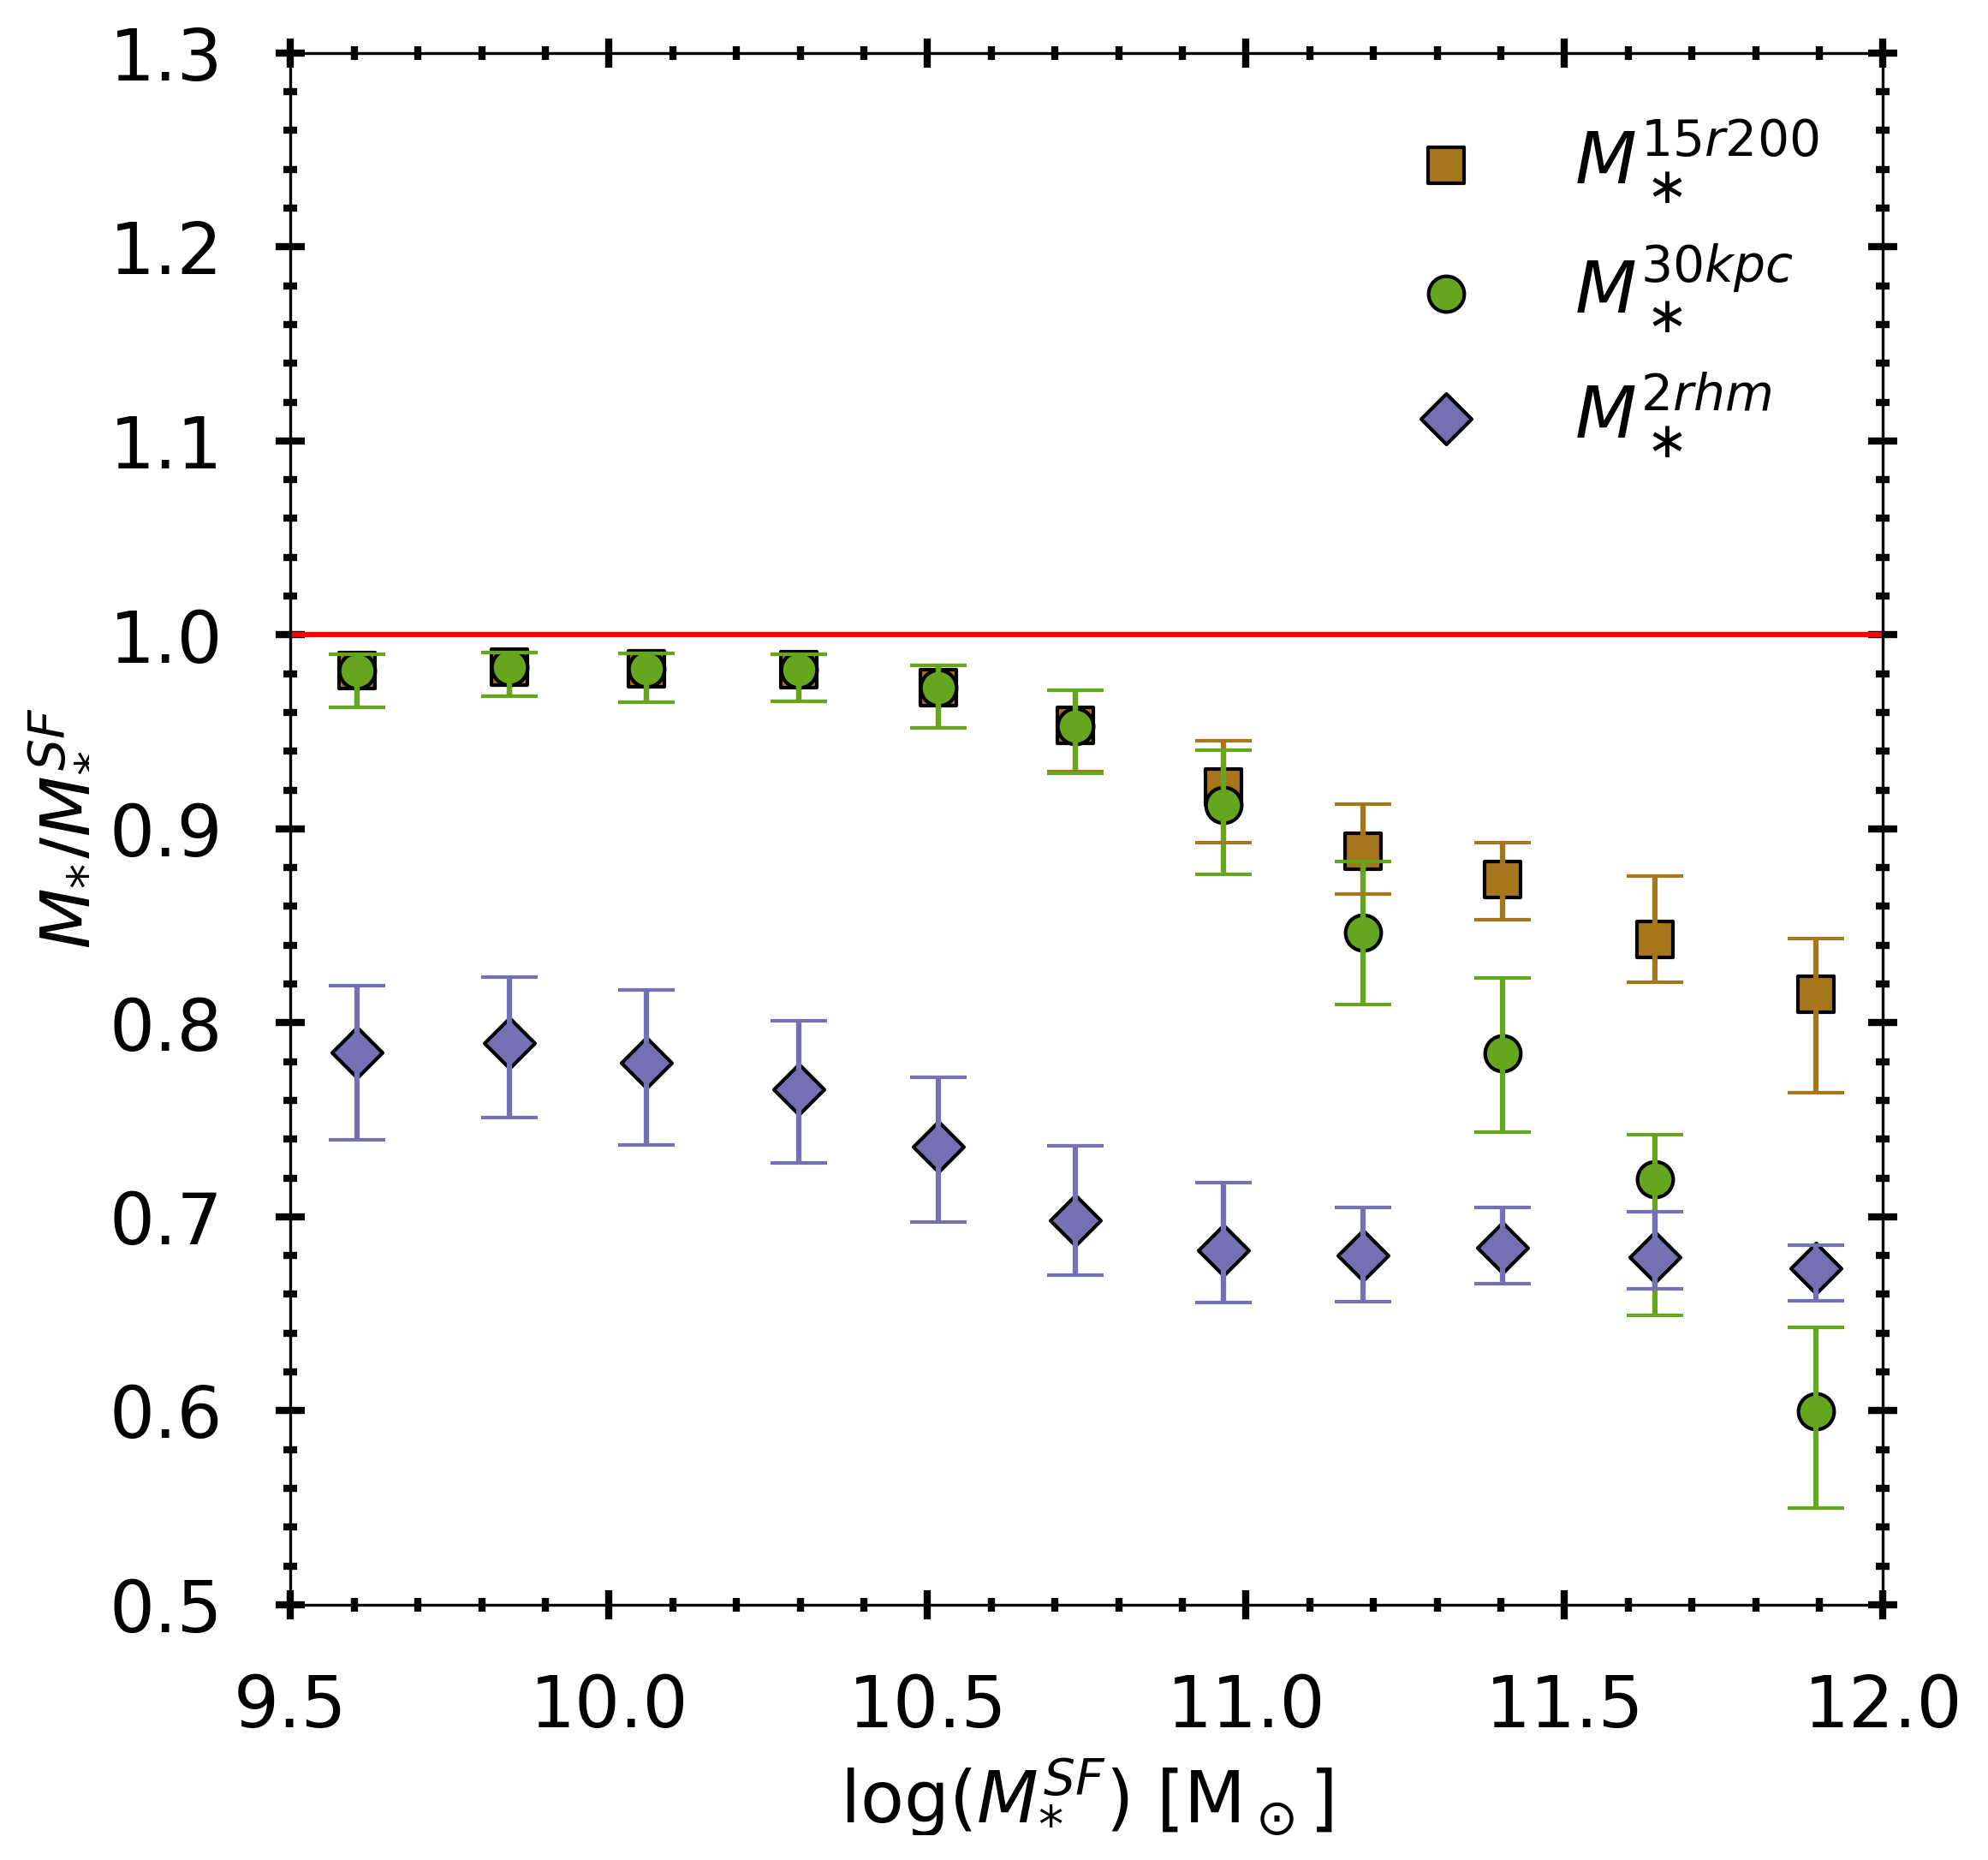
\includegraphics[width=0.9\textwidth]{images/SM_fSM.png}
    \caption{The fractional difference between the stellar mass of the galaxy using different definitions of galaxy size and the total mass of all stellar particles bound to the subhalo as identified by SUBFIND. Median values with 25-75 percentile error bars are given for the stellar mass within 15 \% of the virial radius ($M_\ast^{15r200}$, orange squares), within 30$\,$ kpc ($M_\ast^{30kpc}$, green circles) and within twice the SUBFIND half mass radius ($M_\ast^{2rhm}$, purple diamonds)}
    \label{SM_fSM}
\end{figure}


In Figure \ref{shmr} the SHM relation is shown for the different definitions of stellar mass in TNG ($M_\ast^{15r200}$ is left out to make the figure more readable) along with the best fits from \textcite{Behroozi2013} and \textcite{Zanisi2019}. By using the 30 kpc aperture when calculating the stellar mass for TNG galaxies, the results are more similar to the most recent observations. $M_\ast^{2rhm}$ deviates the most from the slope of the observational data, neither matching the low nor high mass end. This showcases the importance of making it clear which stellar mass definition was chosen, as they do give different results in the SHM relation. However, all the different definitions explored here overestimate the stellar mass compared to observations when looking at the very largest galaxies, even the 30 kpc aperture that undoubtely will be too small for the largest galaxies. Comparing with the newer observational data makes the difference much smaller, and within the error estimates, but it should still be considered whether the feedback mechanisms implemented in TNG tend to give the largest galaxies too much stellar mass. 

\begin{figure}
    \centering
    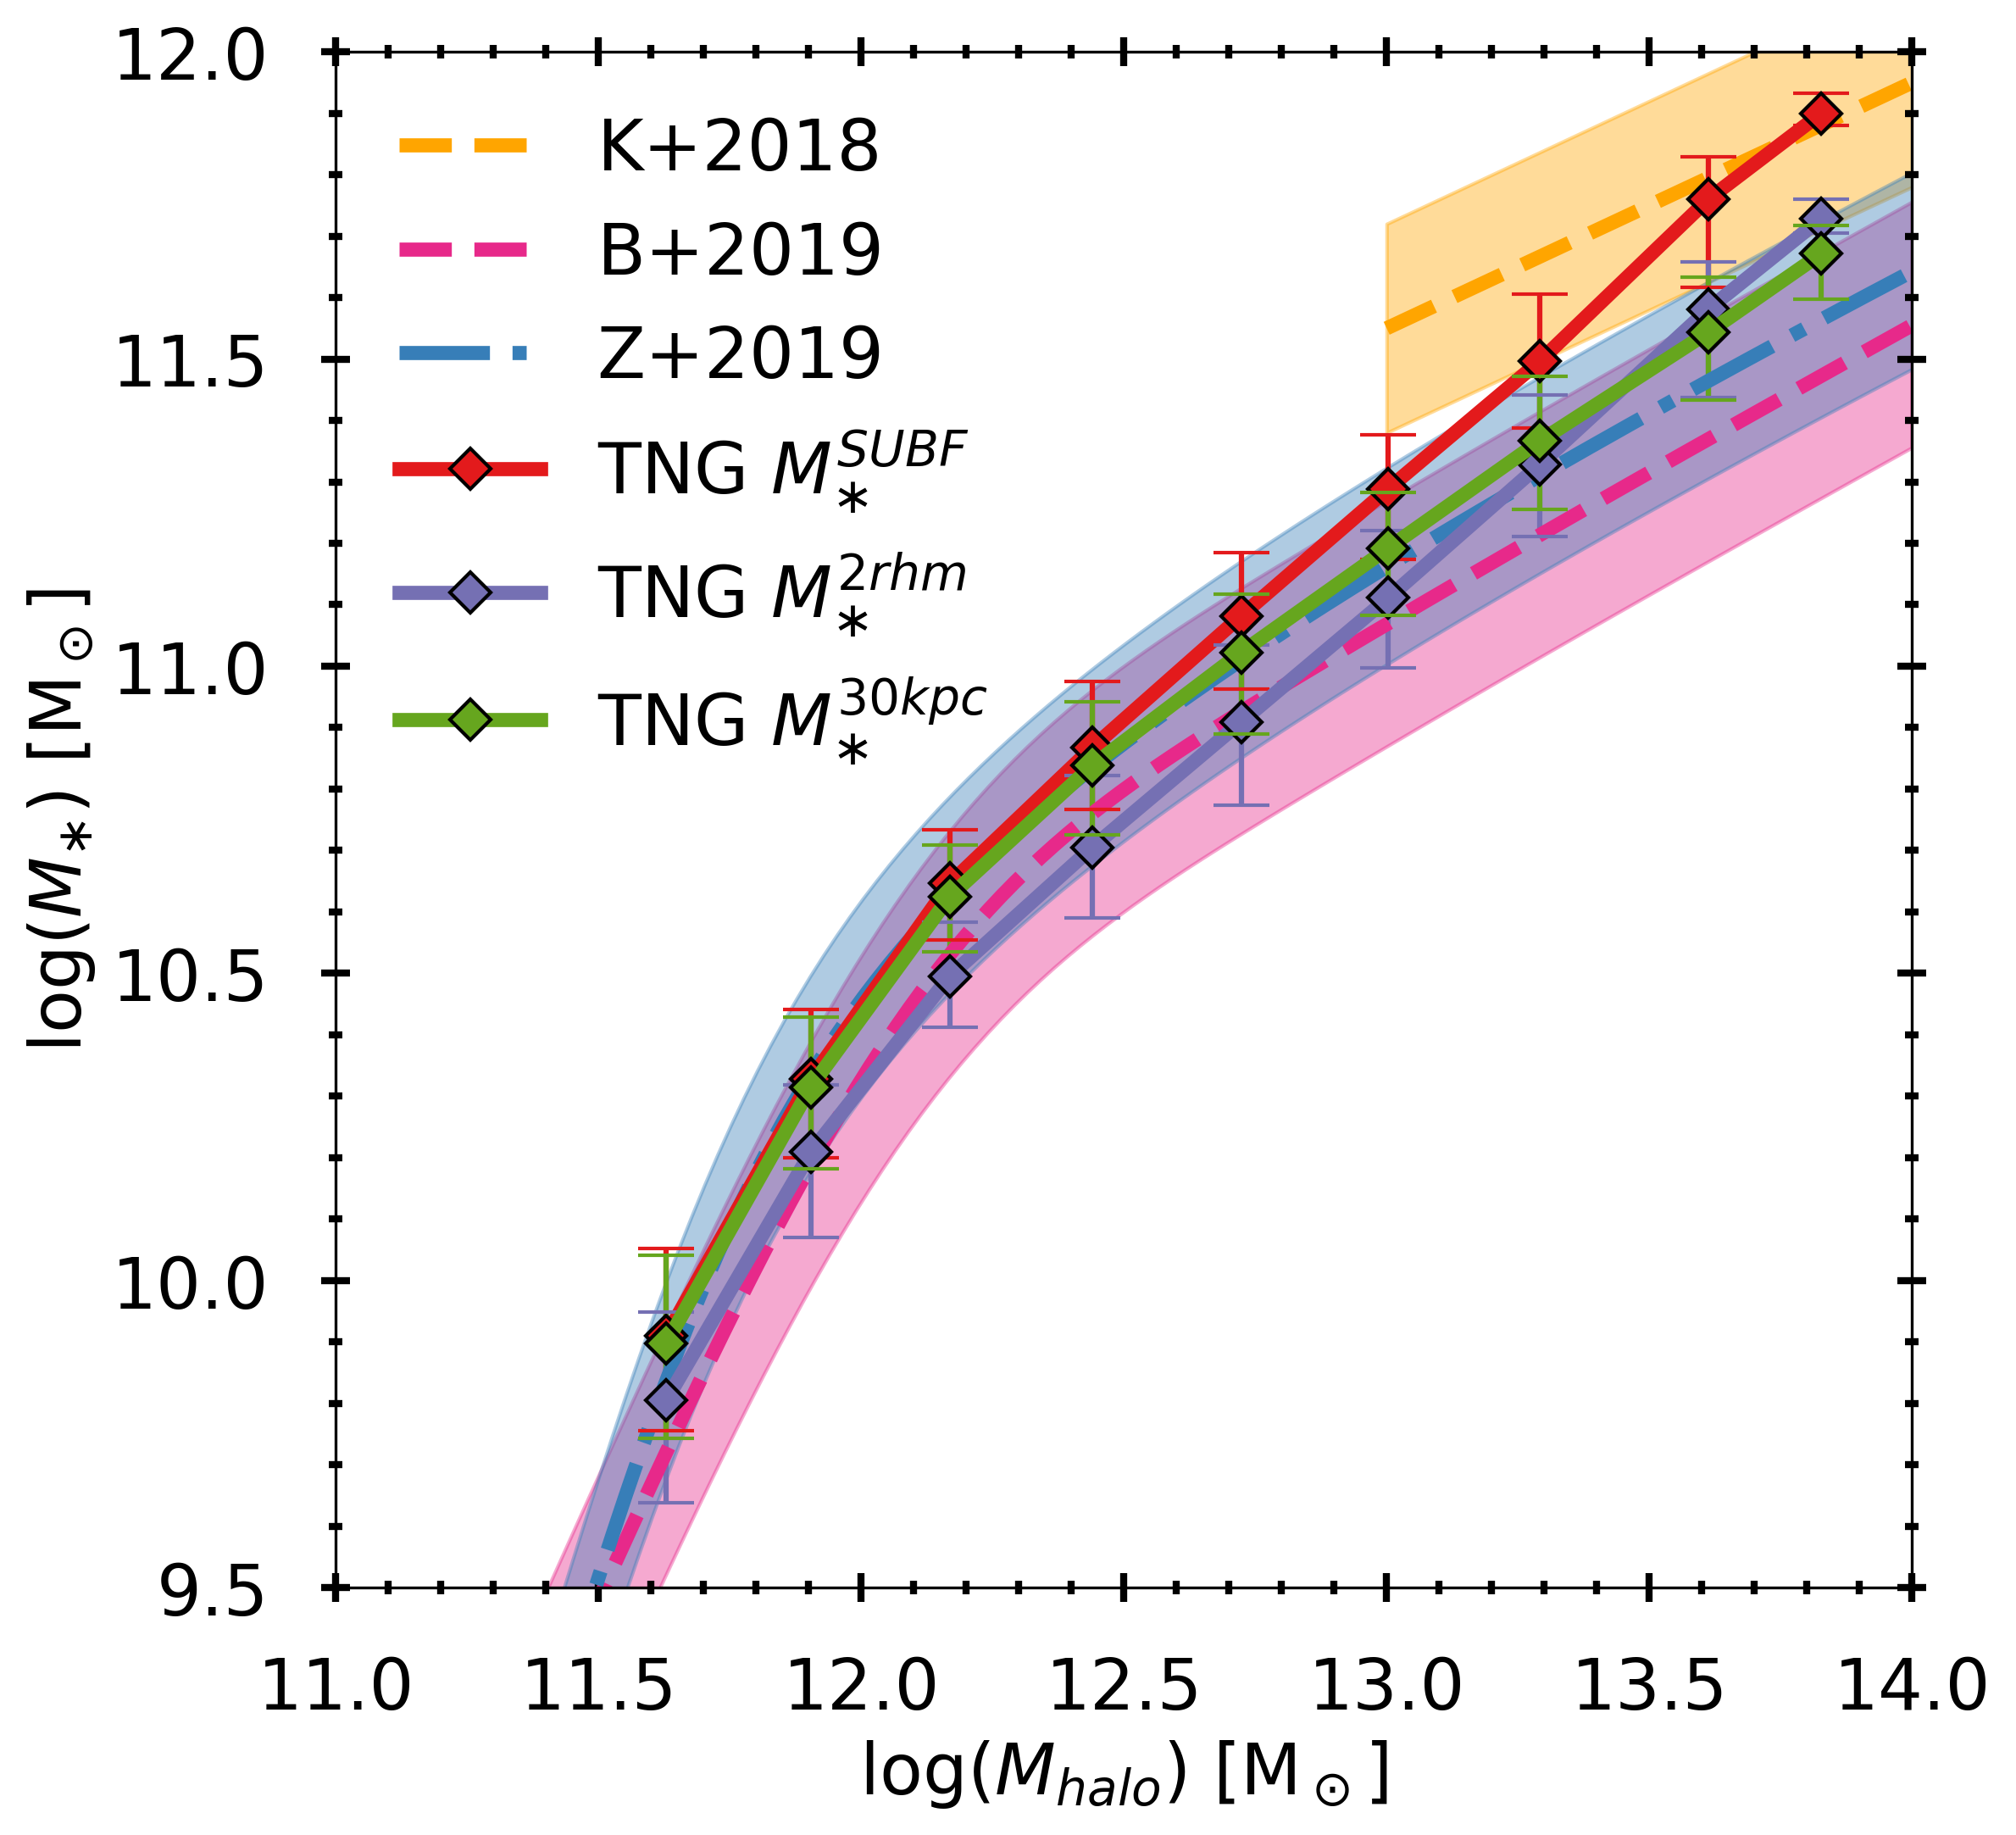
\includegraphics[width=0.9\textwidth]{images/shmr.png}
    \caption{The SHM relation of TNG for three different mass definitions, the stellar mass in the entire subhalo ($M_\ast^{SF}$, red), within 30$\,$ kpc ($M_\ast^{30kpc}$, green) and within twice the SUBFIND half mass radius ($M_\ast^{2rhm}$, purple). The diamond markers indicate median points and include error bars showing the 25-75 percentile. The best fit from abundance matching from \textcite{Behroozi2013} (pink dashed line) and \textcite{Zanisi2019} (orange long-dashed line) are also shown.}
    \label{shmr}
\end{figure}

In conclusion, the stellar masses of TNG galaxies are highly dependent upon the imposed galaxy size limit or lack there of. Compared to observations TNG produces galaxies that are similar in mass for low mass galaxies, but seem to overshoot in the high mass limit.

\subsection{Mass-size-velocity relations}
After looking at the SHM relation, the next fundamental galaxy relations that were studied are those relating to the structure and kinematics of the galaxies. Firstly the stellar mass-size relation gives us an idea about the distribution of the stellar mass within the subhalo. The relation is studied for the entire galaxy population as well as for early and late type galaxies. Next, the velocity measurements of early and late type galaxies as functions of stellar mass give insight into the total mass distribution in the subhalos. Specifically the Tully-Fisher and Faber-Jackson relation are studied and the TNG data are compared against observations.

\subsubsection{Size}
The half-mass radius will of course be affected by the definition of stellar mass, as it is defined as the radius within which half the stellar mass of the galaxy is found. This can be seen in Figure \ref{SM_R_TNG} in which the stellar half-mass radius and the projected half-mass radius is plotted for different galaxy size definitions. There is a large scatter in this function, and the resulting trends lie within the 25-75 percentile of each other. However, it is still clear that there is a difference in the slope of the relation for the $M_\ast > 10^{11} M_{\odot}$ regime. $r^{SF}_{hm}$ is larger than $r^{15r200}_{hm}$ by up to 0.1 dex and larger than $r^{30kpc}_{hm}$ by up to 0.2 dex for the most massive galaxies. 

 It is also interesting to compare the two methods of calculating projected 2D half-mass radii. The only possible method using the SUBFIND catalog is to use the approximate relation $R_{e} \approx 3/4 \times r_{e}$. When using the particles, one can project the galaxies in three orthogonal directions and calculate the average 2D half-mass radius. The results show that multiplying by a factor of $3/4$ is an excellent approximation to the projected stellar half-mass radius.

In Figure \ref{SM_R}, the TNG projected half mass radii for the entire galaxy sample is compared against the data from the SAMI survey. The TNG simulation produces galaxies with half-mass radii that are slightly larger than the SAMI effective radii at lower stellar masses. At high stellar masses the SUBFIND values are higher than those of the fixed aperture of 30 kpc and is a better fit for the Sèrsic-fit effective radius observational data, while $R_{hm}^{30kpc}$ is a better fit for the $R_{e, mge}$ values. TNG galaxies also show a flat or negative slope in the mass range $10^{9.5} M_{\odot} - 10^{10.5} M_{_\odot}$, while the SAMI data has a positive slope such that more massive galaxies have increasingly larger radii across the mass spectrum. This tells us that TNG galaxies become more dense as they grow in size compared to observations, until they reach the characteristic stellar mass $M_\ast = M^{10.5}_{\odot}$, where they again start to expand with increasing mass. It is important to note that there is a large scatter in both observation and simulation results as well as uncertainities which are not accounted for in this study. Keeping this in mind, the similarity in the stellar mass - effective radius relation between observations and TNG is remarkable. 


The stellar mass-size relation for early and late type galaxies is shown in Figure \ref{SM_R_earlies} and Figure \ref{SM_R_lates} respectively. The half-mass radii for late type galaxies are larger than for early types with similar mass, as expected. The relation is sensitively dependent on the criteria used in morphology classifications. In Figure \ref{SM_R_earlies} the SAMI early type galaxies show different behaviours for different morphology classifications in the low mass range. Including the S0 galaxies smoothes out the curve. The galaxy sample is very small in this range though, so this might just be statistical deviations in the mean values. For TNG, the relation does not change significantly based on whether or not the $\kappa_{rot}$ criteria is used. 
For late type galaxies however (Figure \ref{SM_R_lates}) there is a big difference in TNG data. The galaxy sizes of the least massive galaxies increase when the $\kappa_{rot}$ criteria is added. For SAMI data the opposite happens when ``early spirals'' are included in the late type category, the size goes down. This is expected, as more spherical galaxies are smaller than disk-shaped galaxies. Thus, the SAMI ``early + late spirals'' and the TNG $\log(sSFR) > -1.44$ sample are the most similar in the late type size-mass relation. For the early type size-mass relation, the TNG morphology criteria does not matter, but the ``elliptical + S0'' SAMI sample matches better the TNG data.


\begin{figure}
    \centering
    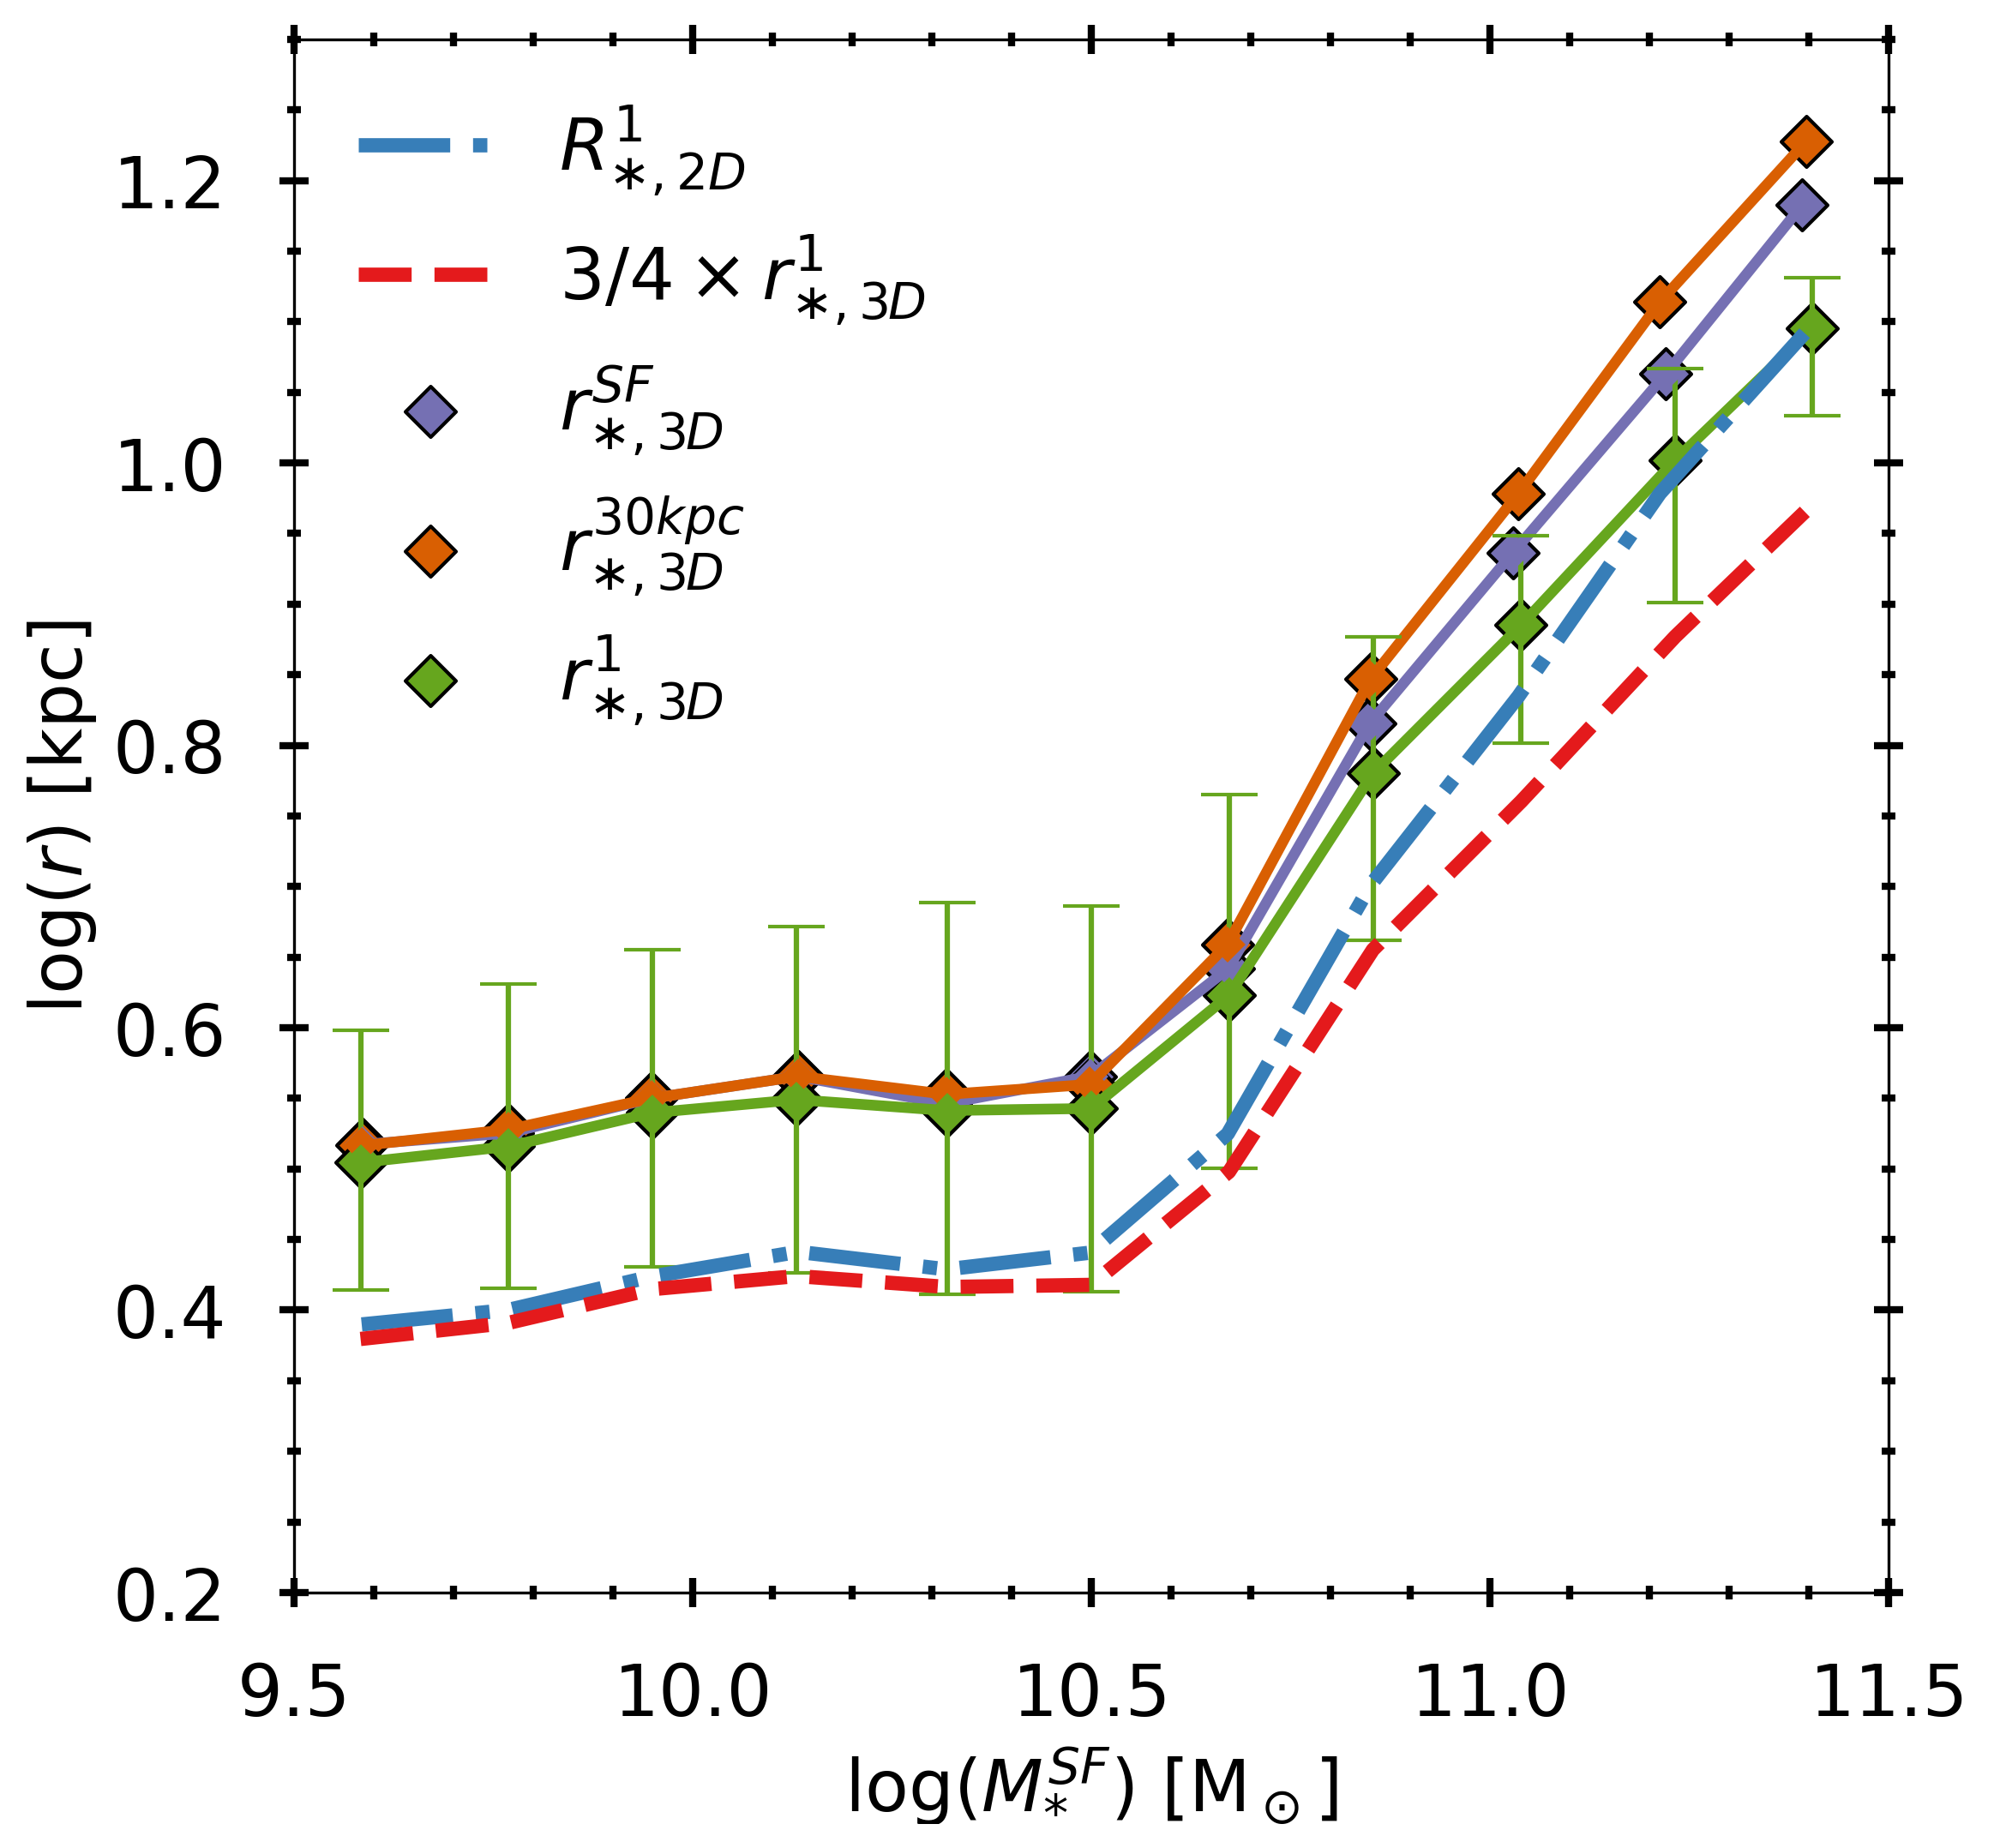
\includegraphics[width=0.9\textwidth]{images/SM_R_tng.png}
    \caption{The size-mass relation for three different galaxy size definitions in TNG, the half-mass radius for the stellar mass in the entire subhalo ($r_{hm}^{SF}$, red), the stellar mass within 15 \% of the virial radius (($r_{hm}^{15r200}$, red), orange squares), within 30$\,$ kpc (($r_{hm}^{30kpc}$, red), green circles). The half-mass radii are all plotted as functions of the total SUBFIND stellar mass $M^{SF}_\ast$. The 2D projected radius $R_{hm}^{15r200}$ and the estimated 2D projected radius $3/4 \times r_{hm}^{15r200}$ are also shown as purple and green dashed lines respectively. The 25-75 percentile error bars are shown for $r^{15r200}_{hm}$ only, as the scatter is similar for all definitions.}
    \label{SM_R_TNG}
\end{figure}


\begin{figure}
    \centering
    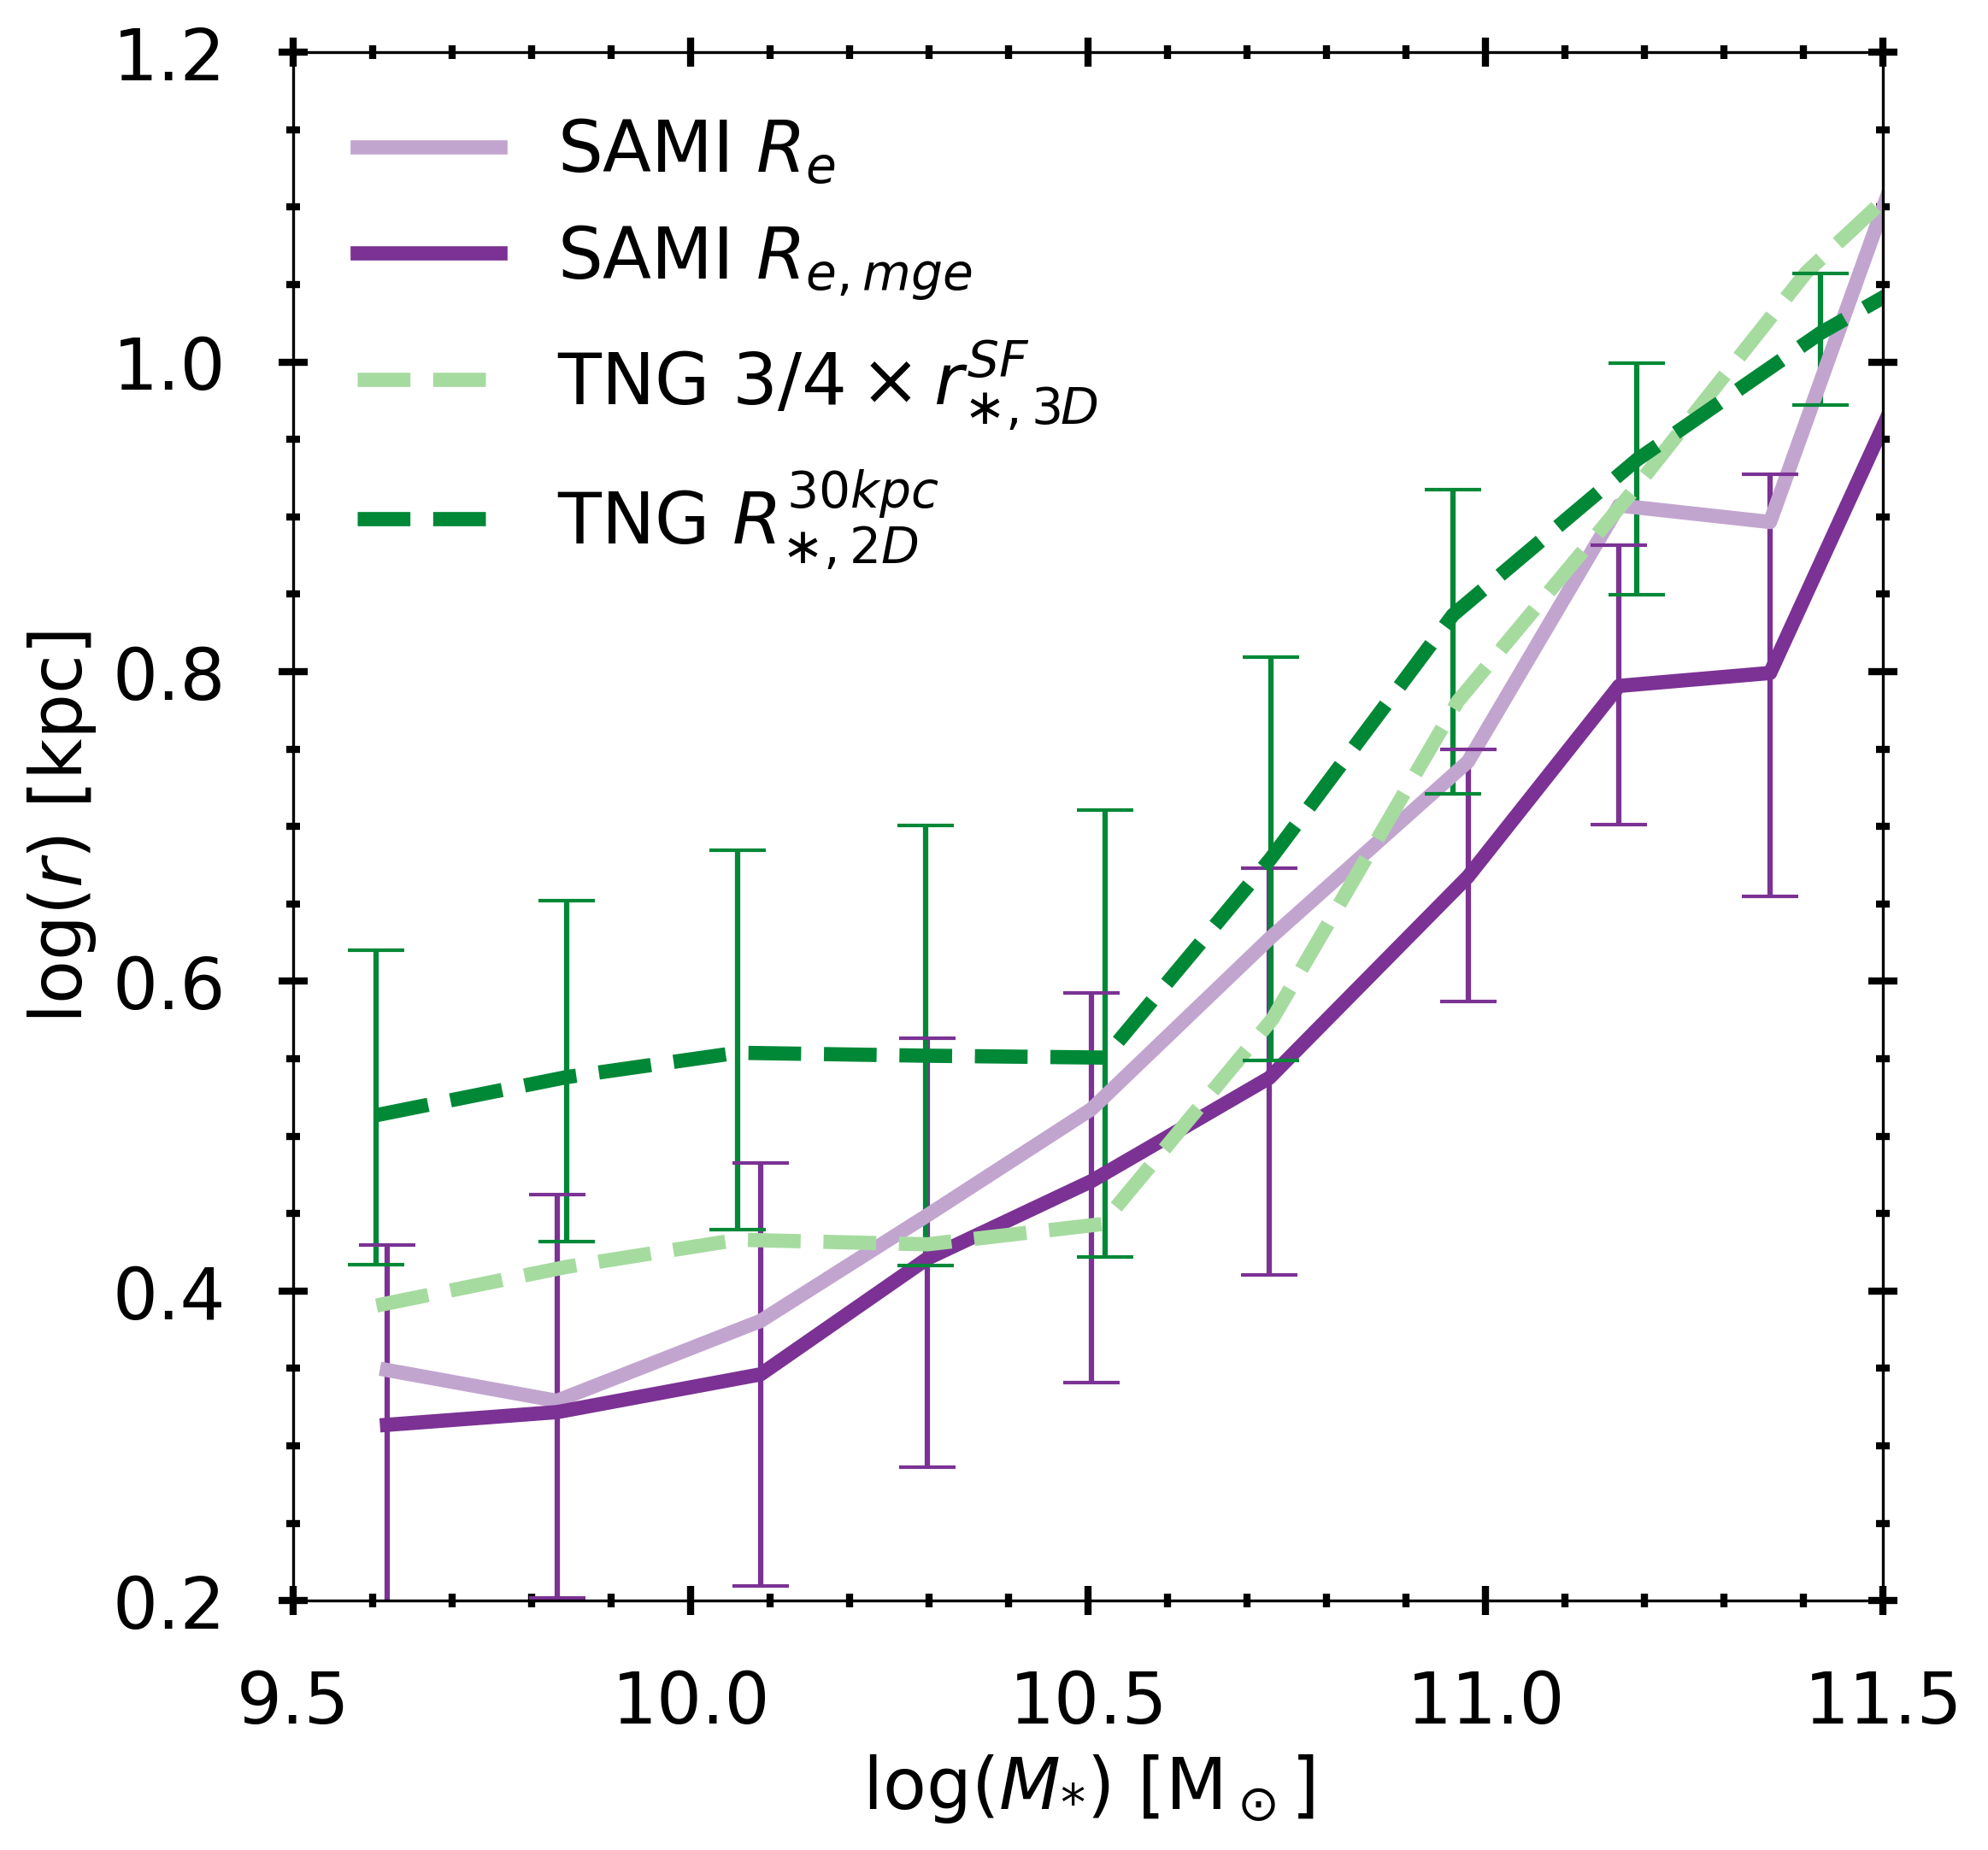
\includegraphics[width=0.9\textwidth]{images/SM_R.png}
    \caption{The size-mass relation of the whole galaxy sample in both TNG and SAMI, given by median values with corresponding 25-75 percentile error bars. TNG values are shown in green dashed lines, while SAMI values are the purple solid lines.}
    \label{SM_R}
\end{figure}

\begin{figure}
    \centering
    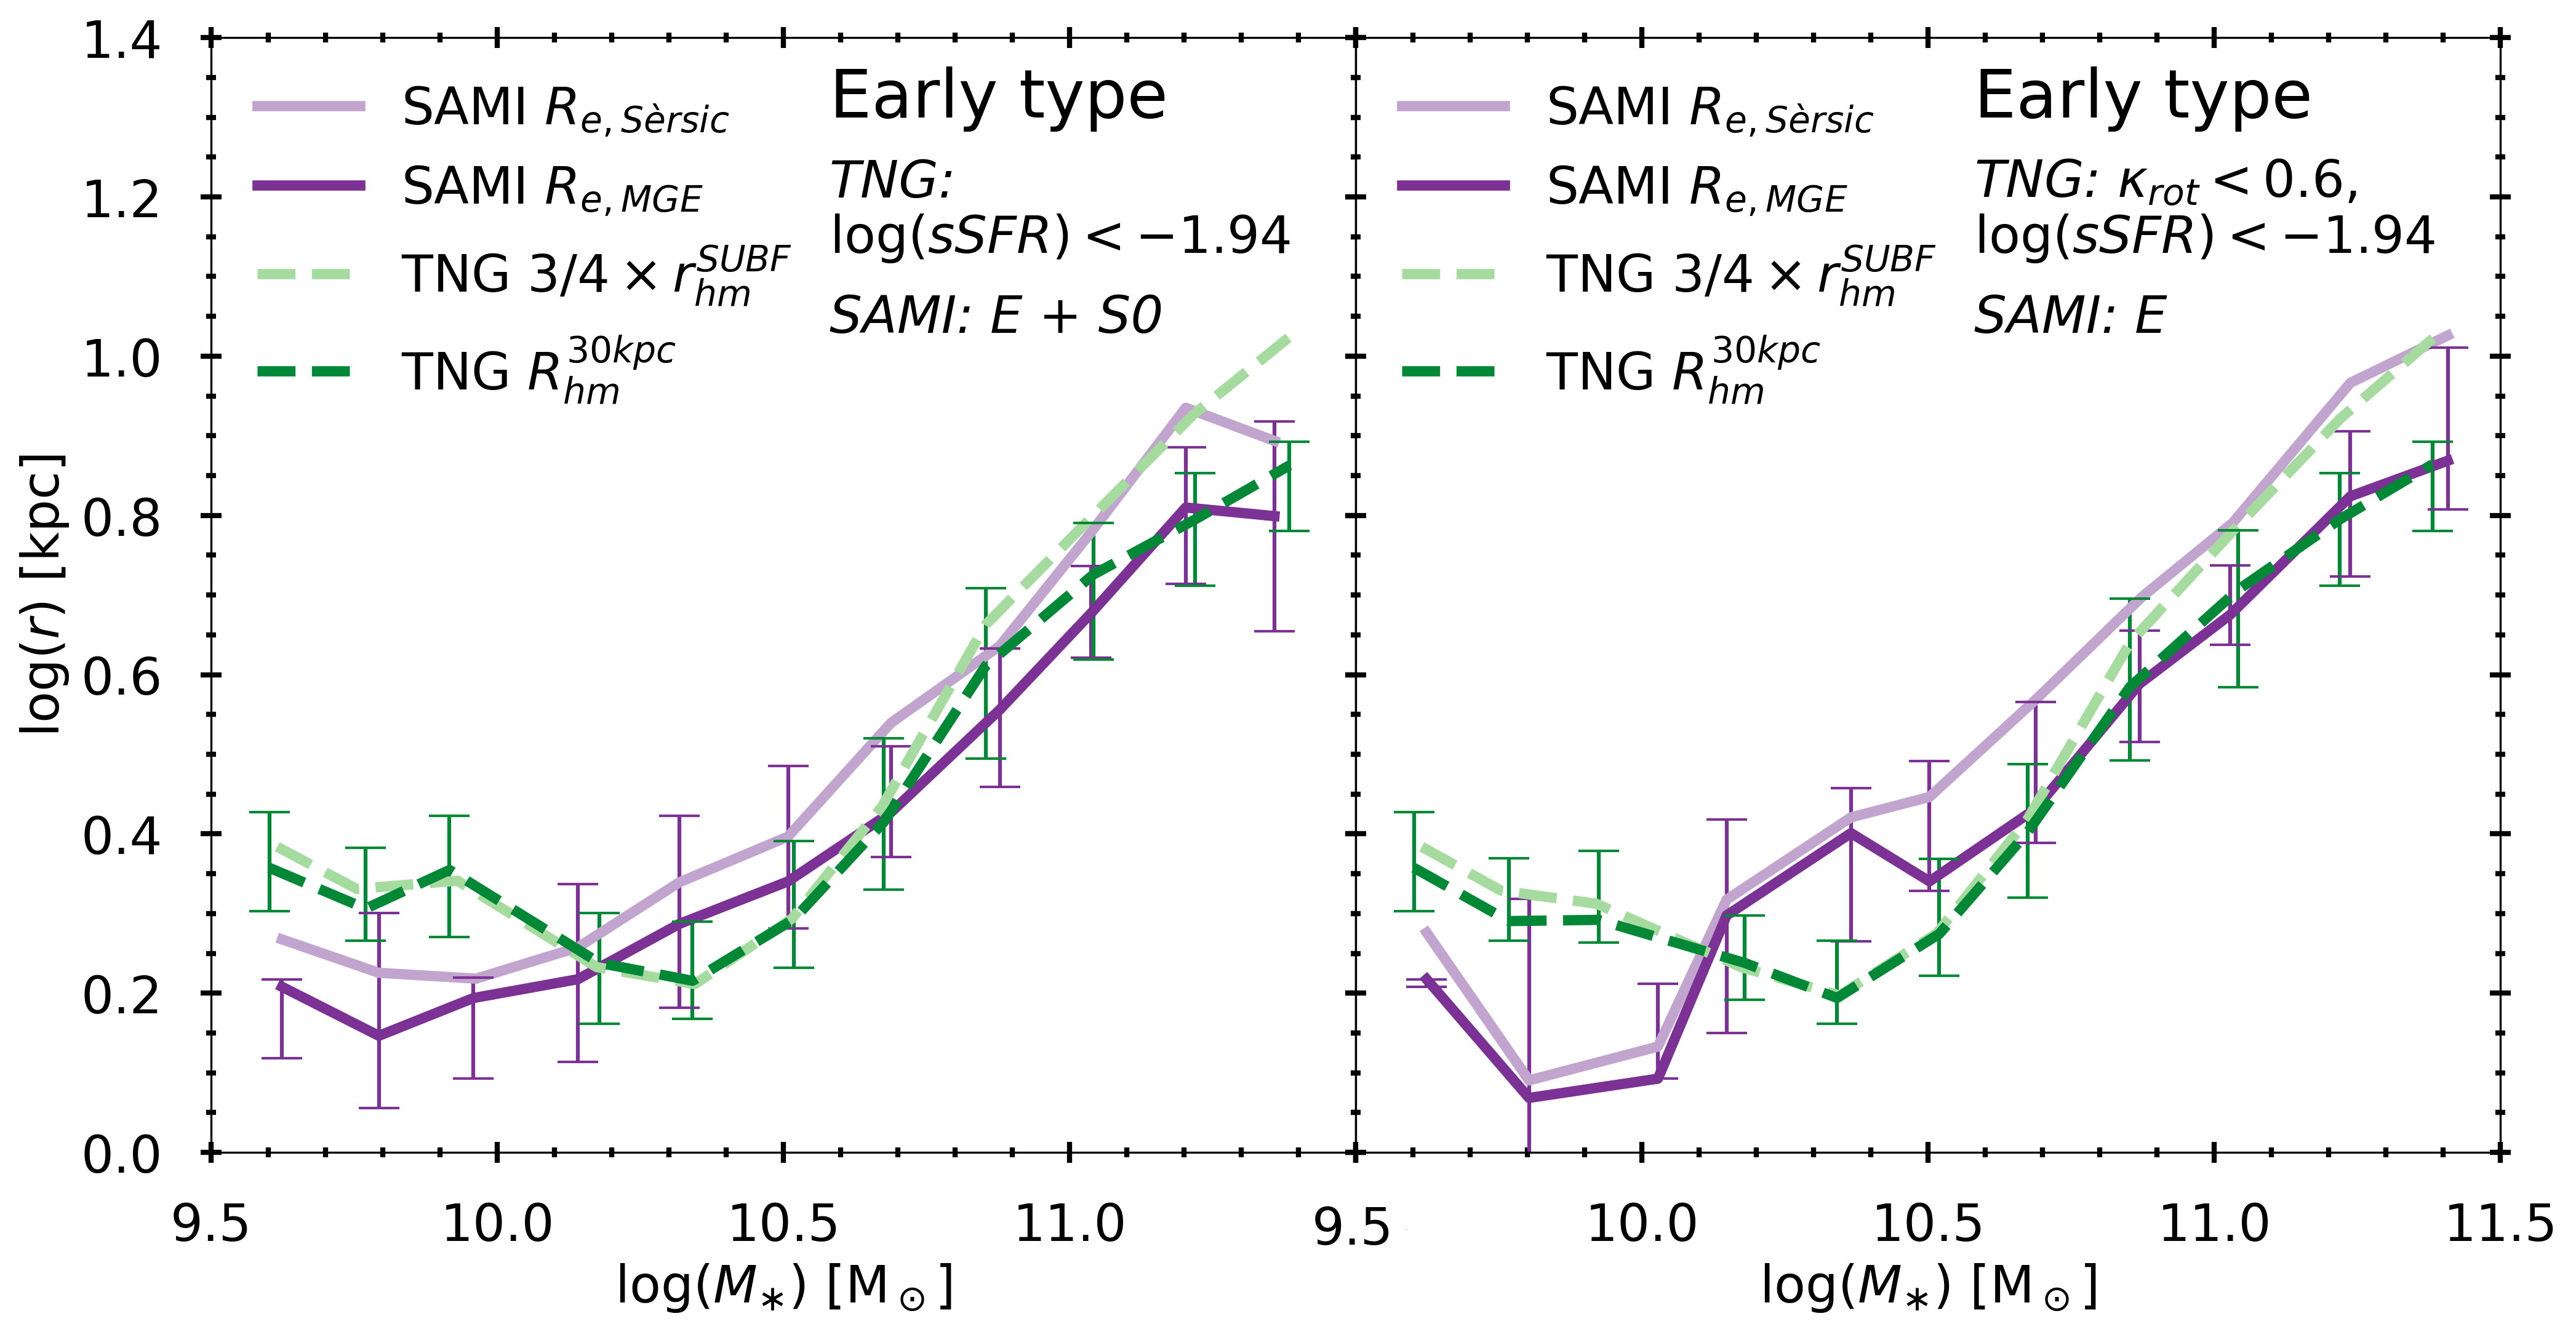
\includegraphics[width=\textwidth]{images/SM_R_earlies.png}
    \caption{The size-mass relation of early type galaxies in both TNG and SAMI, given by median values with corresponding 25-75 percentile error bars. TNG values are shown in green dashed lines, while SAMI values are the purple solid lines. The two panels show the effect of the morphology selection criteria. Left: TNG galaxies with $\log(sSFR) < -1.94$ and SAMI elliptical and S0 galaxies. Right: TNG galaxies with $\log(sSFR) < -1.94$ as well as $\kappa_{rot} < 0.6$ and SAMI elliptical galaxies.}
    \label{SM_R_earlies}
\end{figure}

\begin{figure}
    \centering
    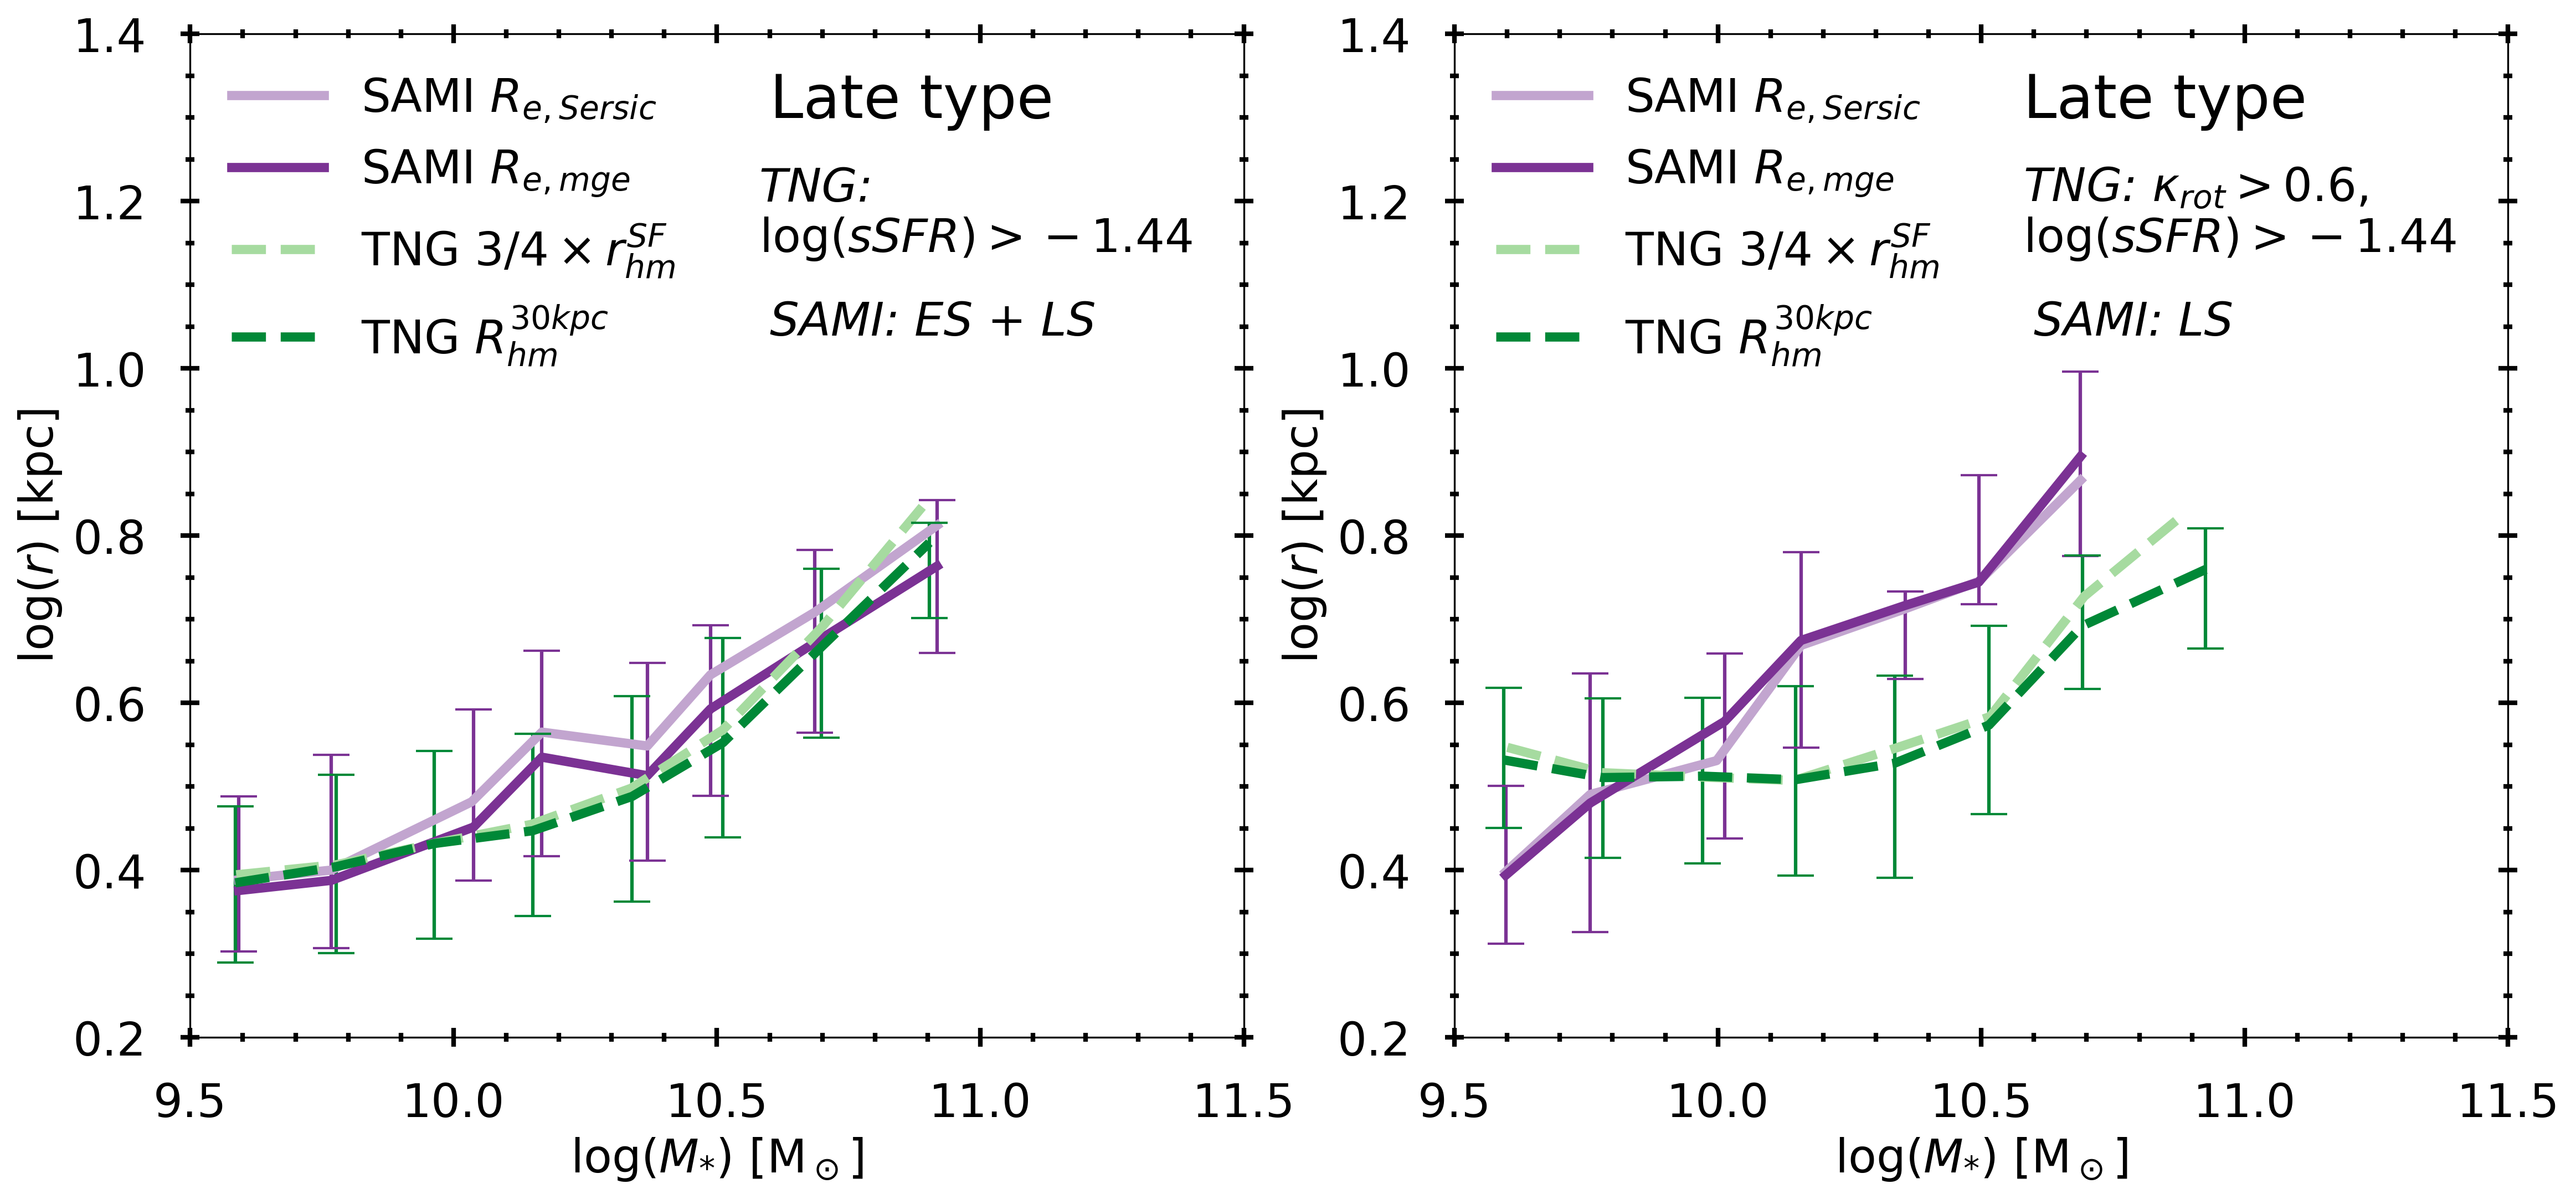
\includegraphics[width=\textwidth]{images/SM_R_lates.png}
    \caption{The size-mass relation of late type galaxies in both TNG and SAMI, given by median values with corresponding 25-75 percentile error bars. TNG values are shown in green dashed lines, while SAMI values are the purple solid lines. The two panels show the effect of the morphology selection criteria. Left: TNG galaxies with $\log(sSFR) > -1.44$ and SAMI early and late spiral galaxies. Right: TNG galaxies with $\log(sSFR) > -1.44$ as well as $\kappa_{rot} > 0.6$ and SAMI late spiral galaxies.}
    \label{SM_R_lates}
\end{figure}

\subsubsection{Rotational velocity}
As the SUBFIND catalog value for rotational velocity is the maximum of the spherically averaged rotation curve, it was interesting to see if the rotational velocities are significantly smaller at specific radii where observational measurements are made. To test this, the rotational velocity was calculated at a distance of $2.2 \times r_{hm}$. There was no difference in the produced data. At that distance the velocity curve is well into the flat regime caused by the dark matter halo, and so this shows that the maximum rotational velocity is not much different from the flat part.

In Figure \ref{TFR} the Tully-Fisher relation is shown for TNG, along with the best-fit from the SAMI data by \textcite{Bloom2017} and \textcite{Bekerait2016} who calculated their velocities at $2.2 \times R_e$ and at the radius within 83\% of the light is contained respectively. Both measurements are within the flattened part of the velocity curve, and so they should be comparable. The TNG data is calculated using a galaxy size of 30 kpc and rotational velocities measured at $2.2 \times r_{hm}^{30kpc}$. The SAMI data has a steeper slope than the TNG data, being 0.31 $\pm 0.1$ and 0.25 respectively. The CALIFA study has a slope of 0.27 $\pm 0.13$, but a lower zero point, and so the TNG results lie between the CALIFA and SAMI fits for $M_\ast > 10^{10}M_{\odot}$. As late type galaxies generally do not exceed $M_\ast = 10^{11} M_{\odot}$, we do not expect to see any difference in the TFR for stellar mass definitions $M_\ast^{15r200}$ or $M_\ast^{SF}$ compared to $M_\ast^{30kpc}$. Using the stellar mass measurement within $2 \times r_{hm}^{SF}$ would decrease the slope further, making for an even worse fit to the observational data. The SAMI fit is based on a sample of galaxies that span a mass range of $10^{7.5} M_{\odot} - 10^{11.5} M_{\odot}$, but the TFR extends across the stellar range, with a higher scatter at low stellar masses, so it is still comparable to the TNG data which only spans a range of about $10^{9.5} M_{\odot} - 10^{11} M_{\odot}$. 
\begin{figure}
    \centering
    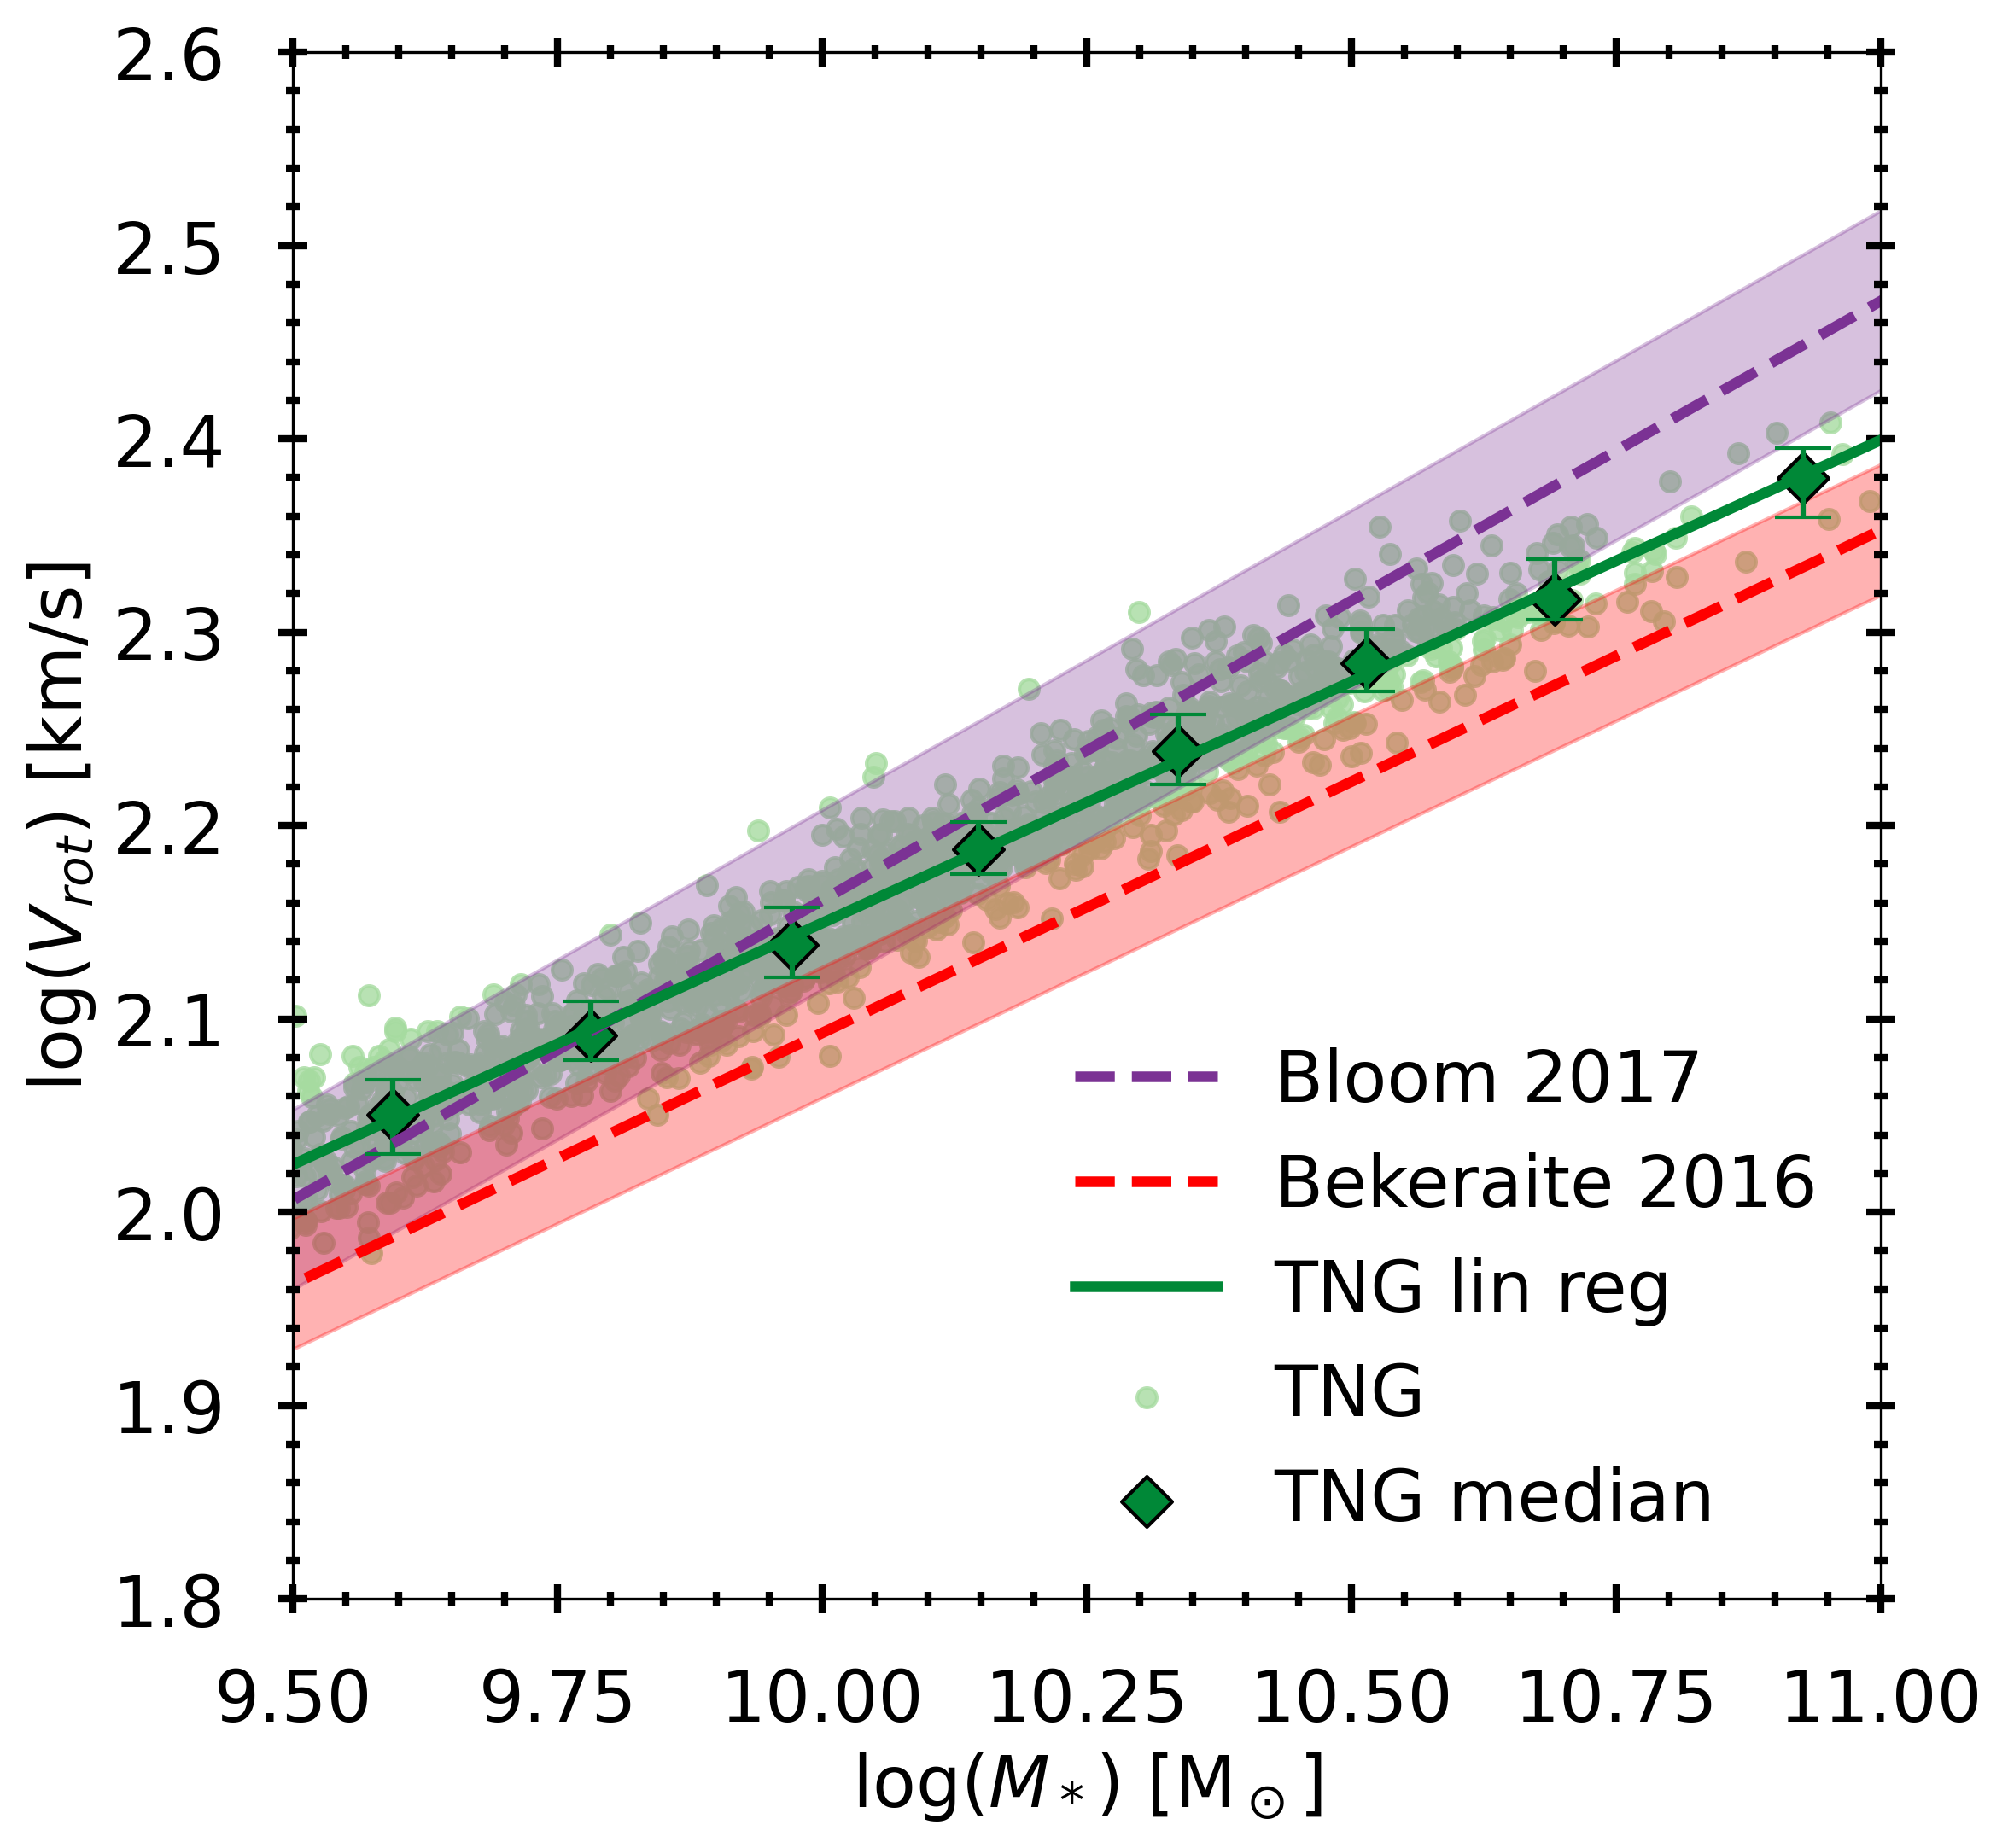
\includegraphics[width=0.9\textwidth]{images/TFR.png}
    \caption{The TFR for TNG (green dots). The median points (green diamonds) for TNG are plotted with error bars, showing the 25-75 percentile. The TNG linear fit is also provided (green solid line). To compare with observations, the best fit for the SAMI data from \textcite{Bloom2017} is shown (purple dashed line) along with the best fit for the CALIFA survey from \textcite{Bekerait2016} (red dashed lline).}
    \label{TFR}
\end{figure}


\subsubsection{Velocity dispersion}
To investigate the difference between using the particles and the SUBFIND catalog for velocity dispersion estimates, several aspects of how velocity dispersion is calculated must be considered. The SUBFIND value is the mass averaged velocity dispersion of all particles that are bound to the subhalo ($\sigma^{SF}$), and is the only velocity dispersion measurement found in the group catalog. The velocity dispersion measured observationally is either that of stars or that of gas, so using this total velocity dispersion might not give comparable results. In Figure \ref{VD_part} the contribution to $\sigma^{SF}$ by stellar, gas and dark matter particles are presented. $\sigma^{SF}$ is the mass averaged sum of these values, and is higher than the baryonic (gas and stars) velocity dispersions because of the contribution by the dark matter that makes up most of the mass in the subhalo. Gas velocity dispersion is lower than $\sigma^{SF}$ by more than 30 \%, and reaching 45 \% in the highest mass galaxies. Thus, using $\sigma^{SF}$ as a proxy for $\sigma_{gas}$ is not advisable. The stellar velocity dispersion is much closer to $\sigma^{SF}$, being approximately equal up to the very largest galaxies where it is less than 10 \% smaller. It is still not ideal to use the SUBFIND values, and this is a good argument for why it is important to use the particles for these kinds of analysis.

Looking further at the stellar velocity dispersion in TNG, the effect of a limit on the galaxy size was studied. This is because it might be assumed that velocity dispersion will fall off in the outer parts of the galaxy, and be higher closer to the center. The results show that there is little to no difference in velocity dispersion values for stellar particles within $0.15 \times r_{200}$ or within 30 kpc compared to the entire subhalo. Observational values are often averaged within $r_e$, so this was also done for TNG, yielding slightly smaller velocities at the high mass end. The projection effect was also studied by calculating the projected velocity dispersion in three orthogonal directions and comparing it to scaling the 3D velocity dispersion by a factor of $1/\sqrt{3}$. The difference was neglible, as expected for the elliptical early type galaxies.

\begin{figure}
    \centering
    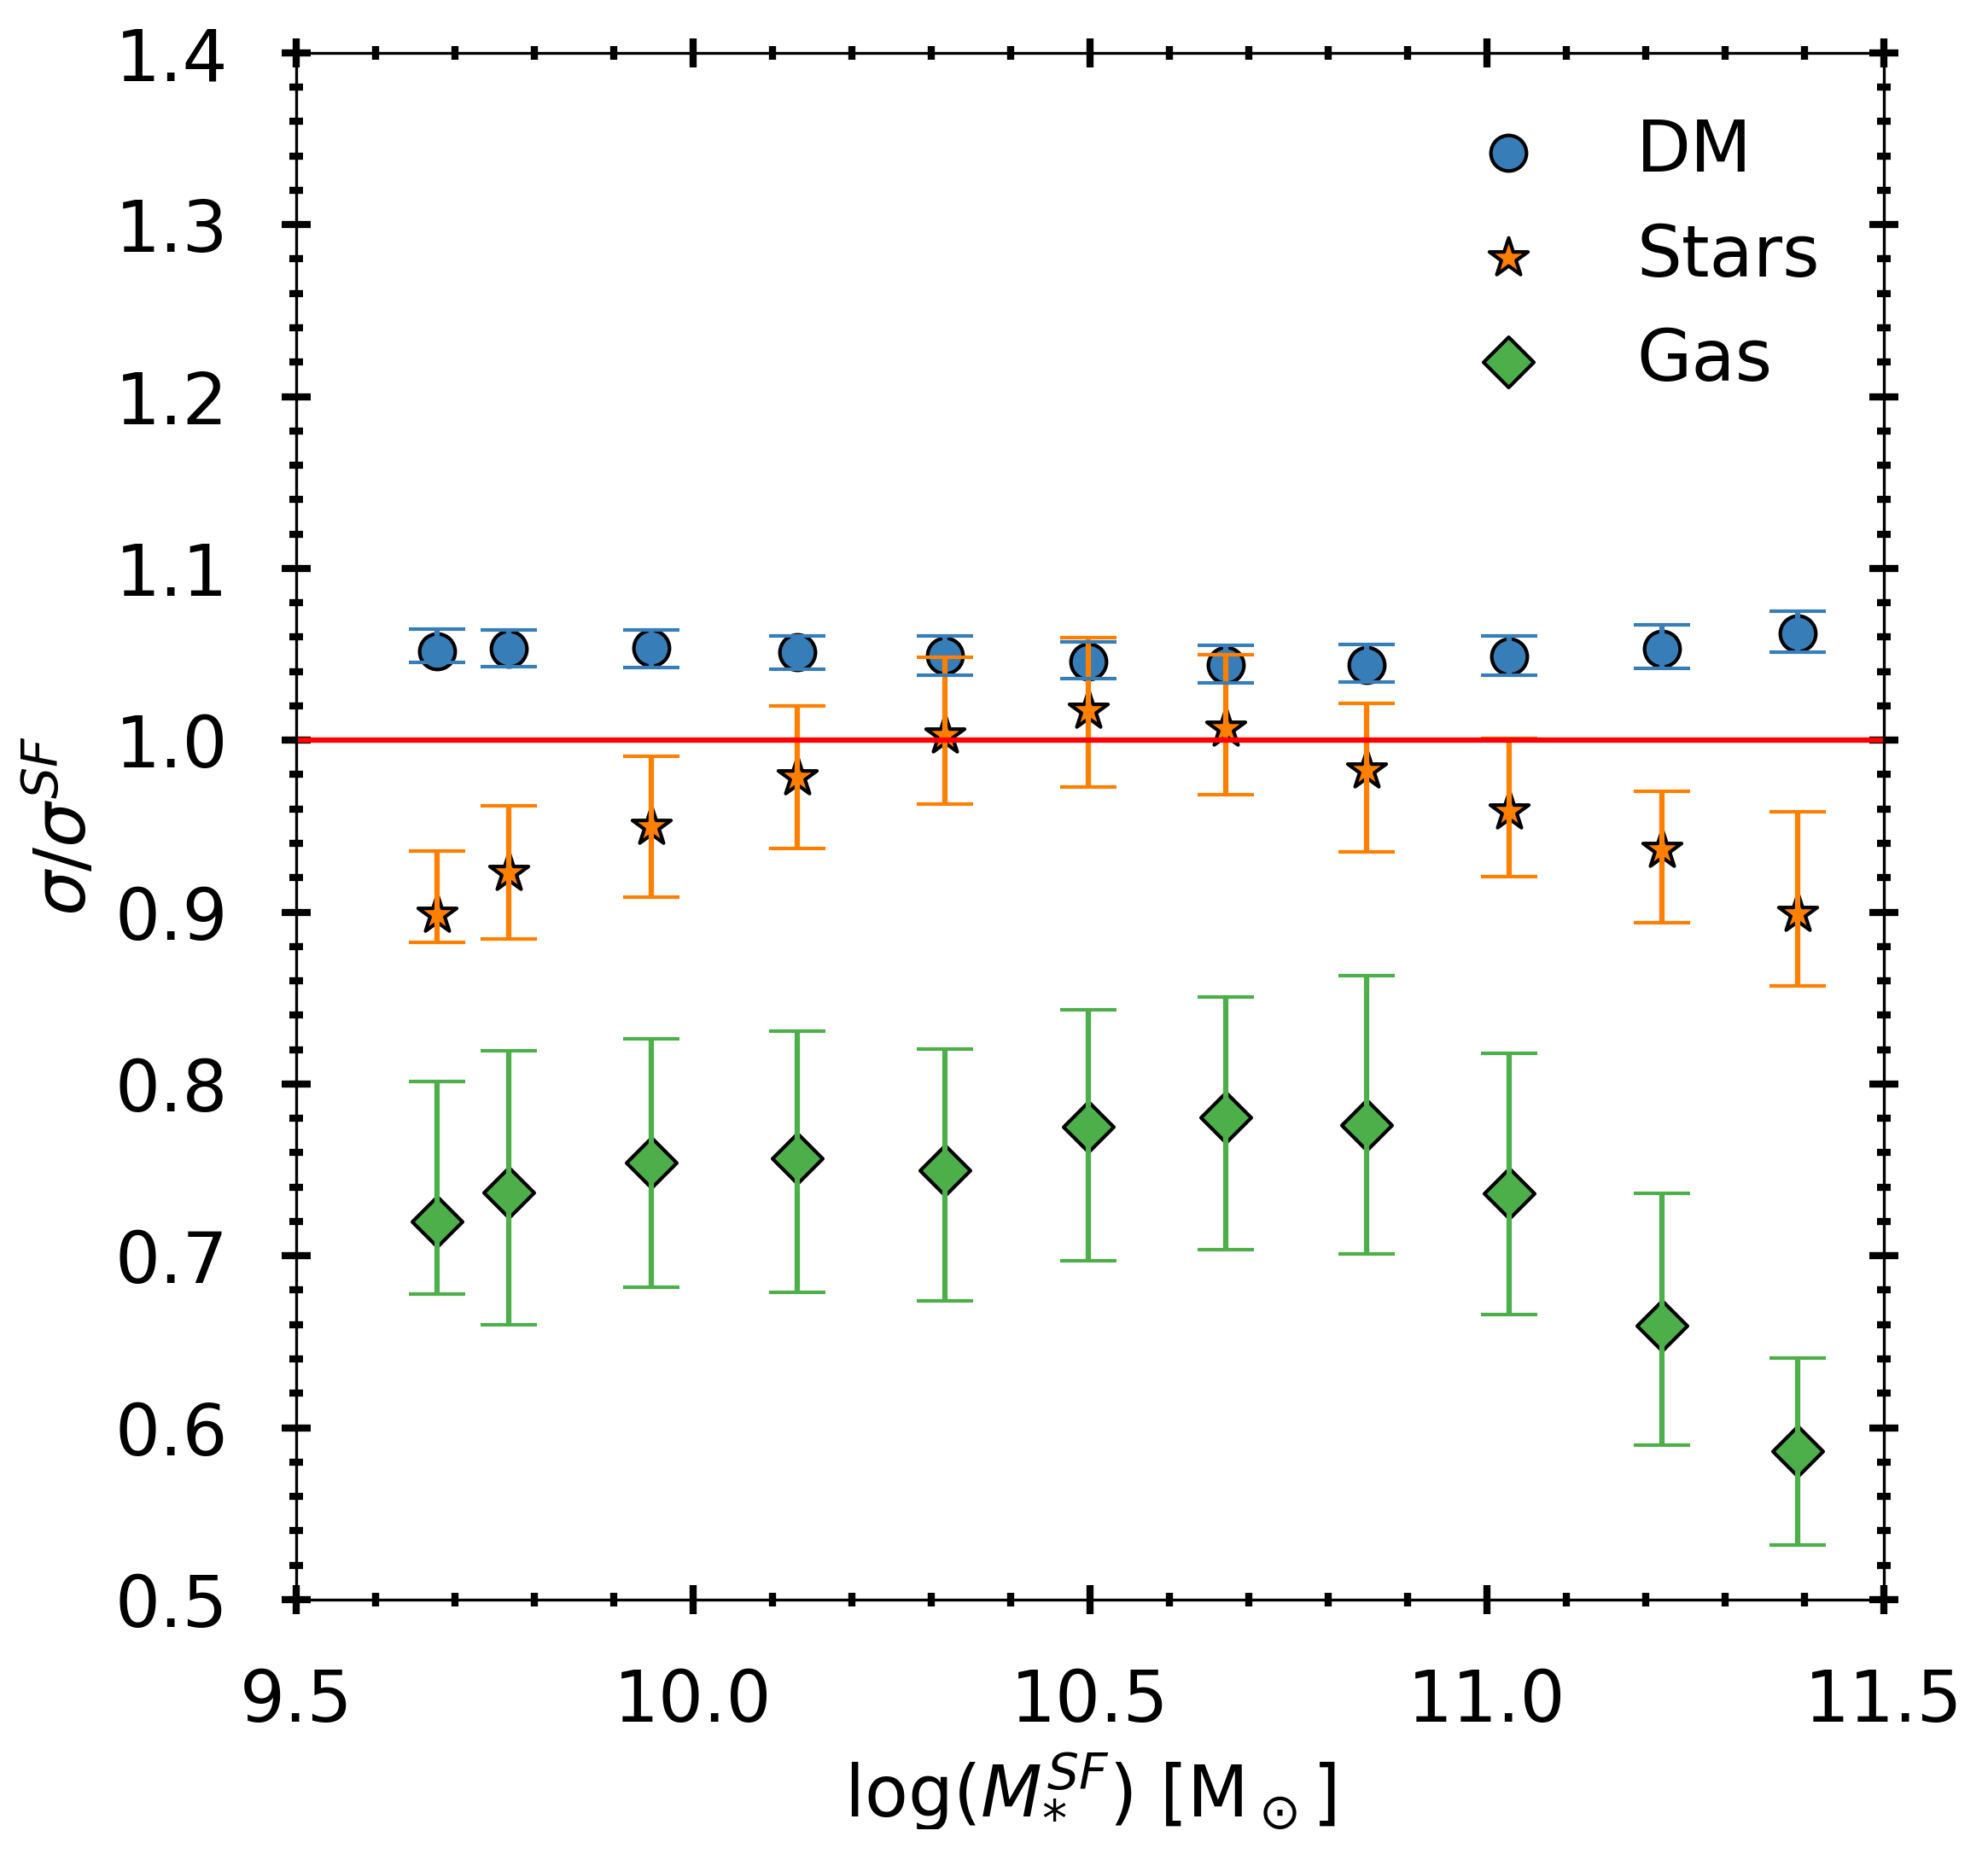
\includegraphics[width=0.9\textwidth]{images/VD_particles.png}
    \caption{Velocity dispersion plotted as function of mass for particles bound to TNG subhalos as identified by SUBFIND. Median values with 25-75 percentile error bars are shown for dark matter (blue circles), stellar particles (orange stars) and gas cells (green diamonds).}
    \label{VD_part}
\end{figure}

The Faber-Jackson relation for early type galaxies is shown in Figure \ref{FJ}. We get lower velocity dispersion in TNG compared to SAMI, by about 0.05 - 0.15 dex. It is tempting to contribute the discrepancy to the difference in stellar mass, however by looking at the SHMR relation in Figure \ref{shmr} we see that the mass deviates from observations at around $10^{11} M_{\odot}$, while in Figure \ref{FJ} the difference starts much earlier. Also, the mass is only off from the observations by about 0.1-0.2 dex, but starting at $10^{10.5} M_{\odot}$ the difference from SAMI in the Faber-Jackson relation is larger, up to 0.4 dex at the highest masses. From this, it would seem that velocity dispersions in TNG are lower than those seen in observations at redshift $z=0$. Based on the above analysis, it does not seem like this can be attributed to projection effects or the size of the volume within the velocity dispersion is calculated, but rather the velocities of the simulated stellar particles are in general lower than that which is observed in the stars of real elliptical galaxies.

\begin{figure}
    \centering
    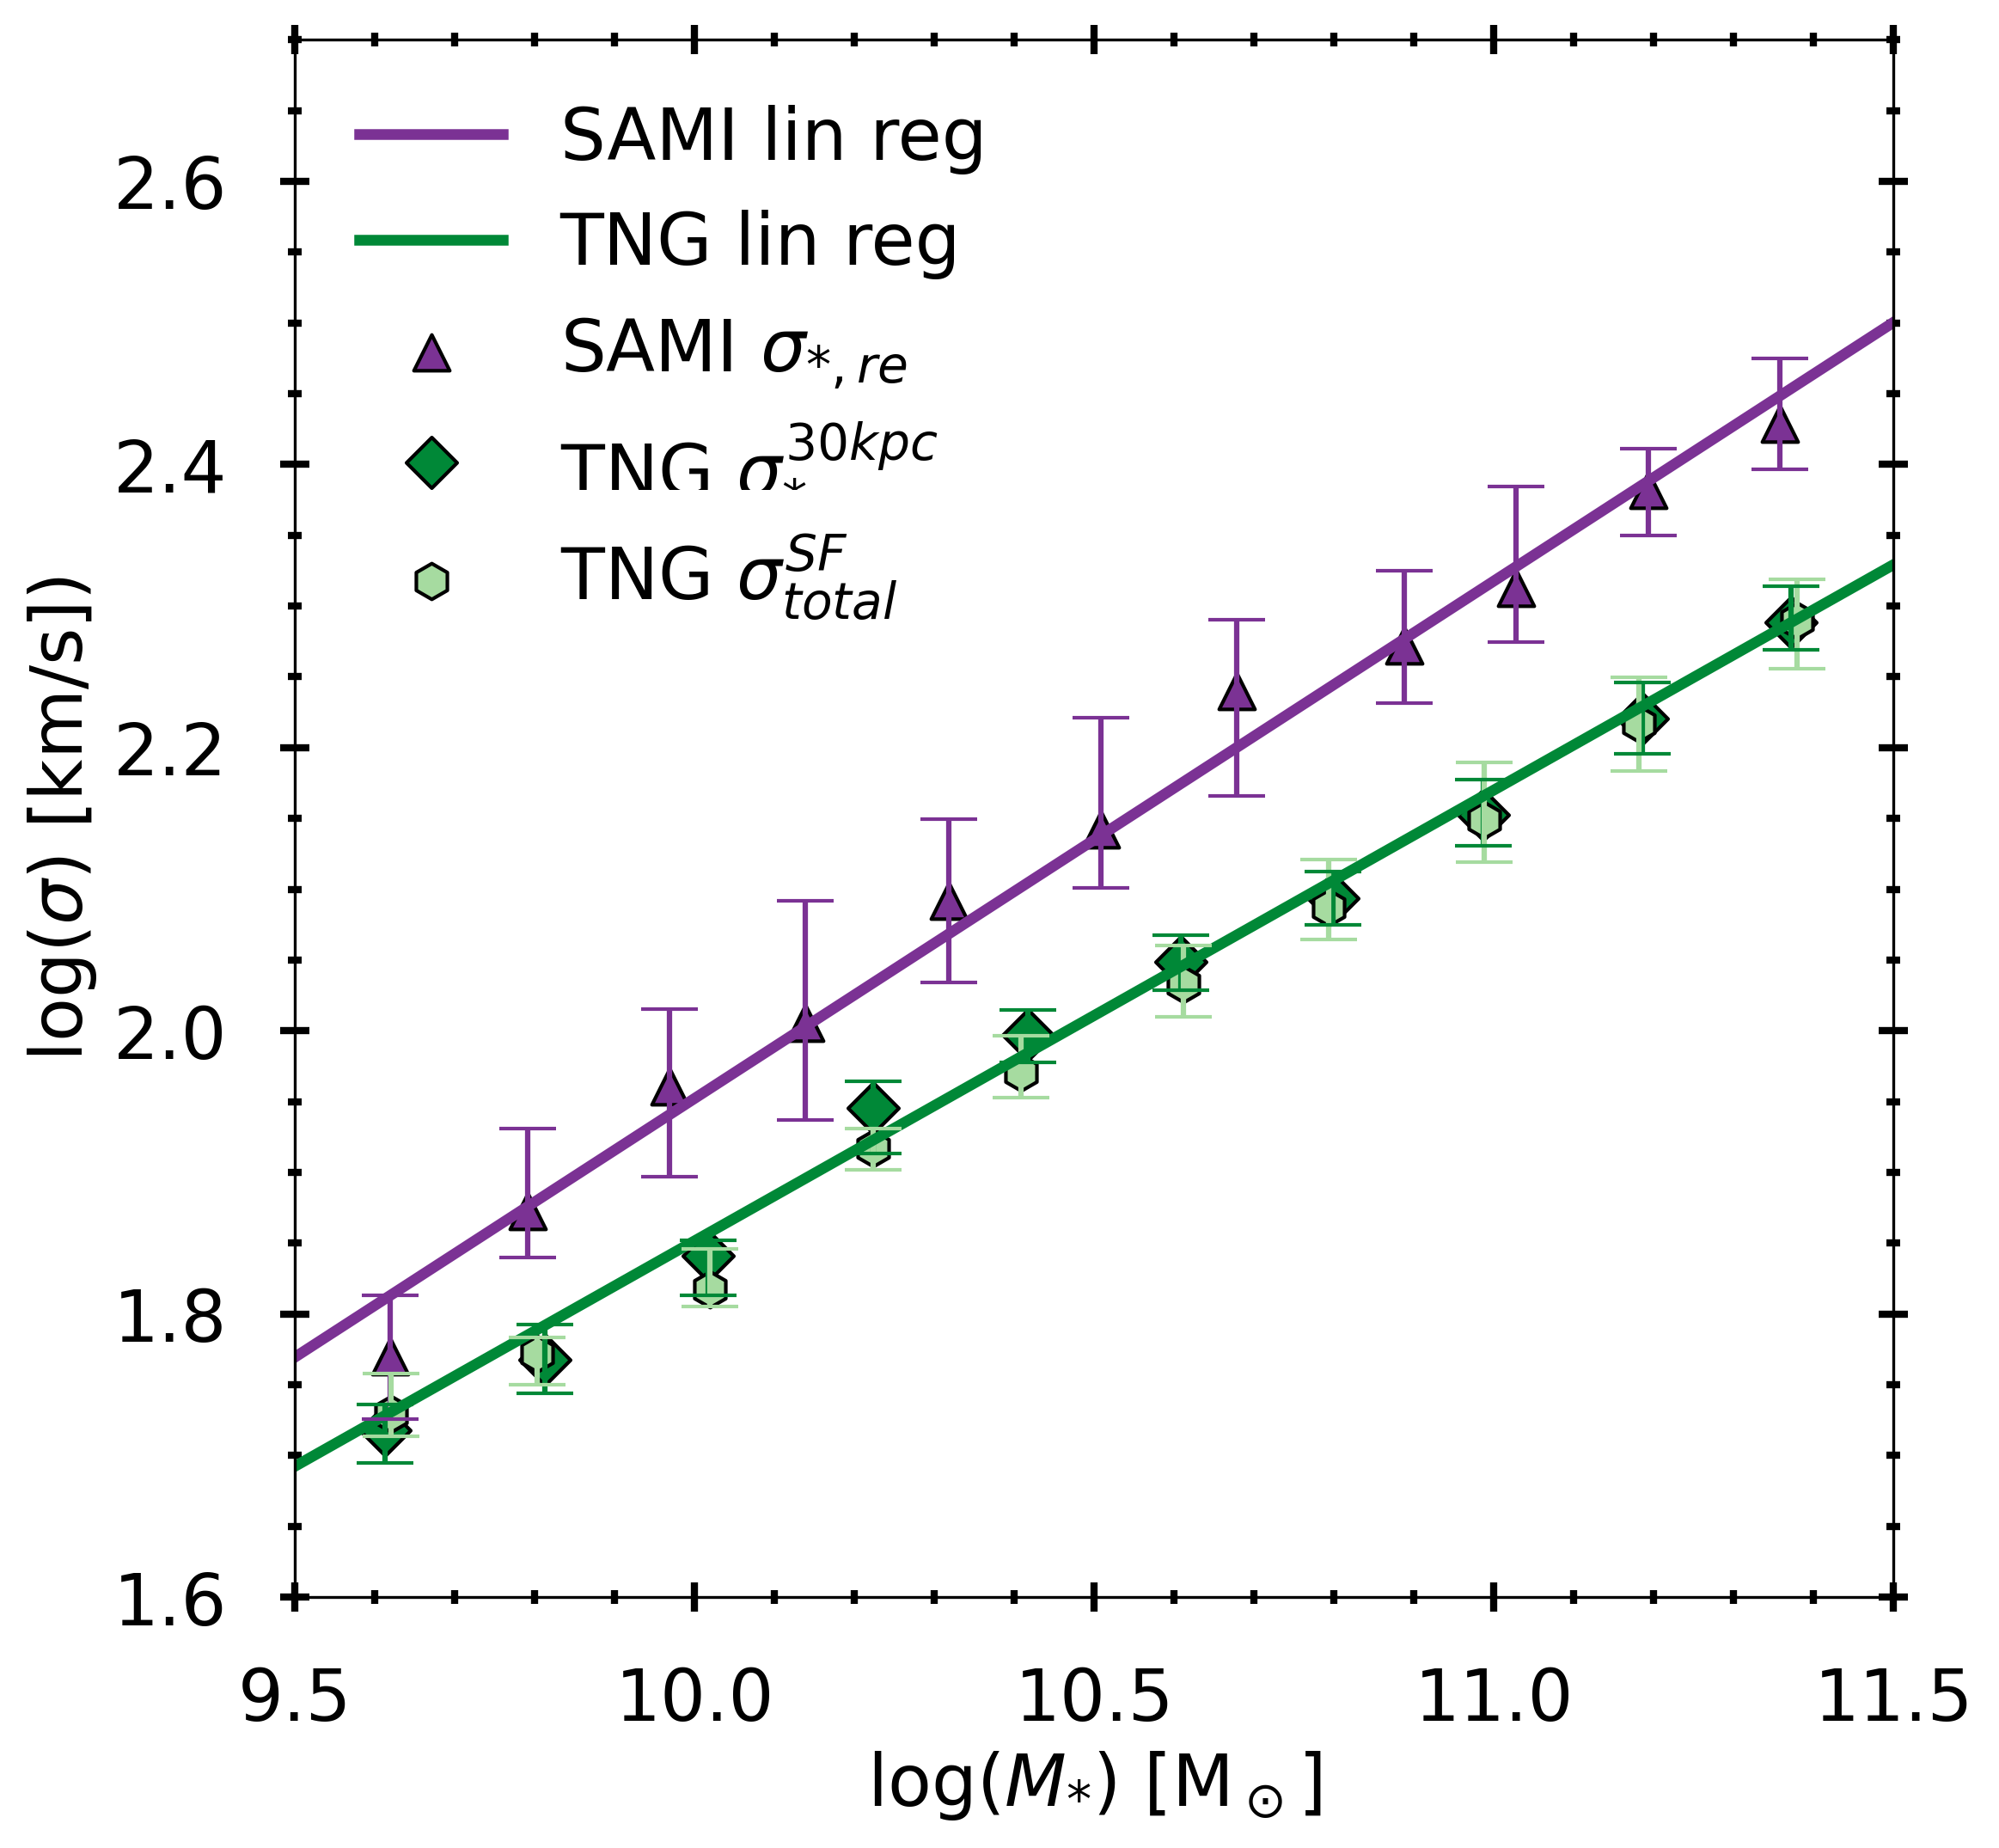
\includegraphics[width=0.9\textwidth]{images/FJ.png}
    \caption{The FJ relation in early type galaxies given by median points with 25-75 percentile error bars for for TNG (dark green points) and SAMI (purple points). Also included are the median points and error bars for the SUBFIND catalog (light green points). The linear fit to TNG (SAMI) are shown as a solid dark green (purple) line.}
    \label{FJ}
\end{figure}

All in all, the mass-size-velocity relations of TNG studied here all show the expected trends found in observational data, but there are some discrepancies especially with the most massive galaxies.

\subsection{Color bimodality}
The final galaxy property which was studied is the color bimodality. Color bimodality is an important feature of observed galaxies, and it has been well documented to be present in TNG galaxies as well \parencite{Nelson2017}. Firstly, the sensitivity to aperture sizes of the g-i color measurements was checked, and there was no apparent difference in the results. This is expected, as the g-i color measures the color of the light that is coming from stars. The larger galaxies, which are the most affected by a limiting aperture, are made up of old stars with very little star formation going on regardless of which part of the galaxy is inspected. The results presented in this section are therefore those measured within the 30 kpc aperture, as those stellar masses are closer to the observed values in the SHMR. It is also important to mention here that SAMI data contains satellite galaxies as well as centrals, so they will be more affected by environment than TNG galaxies.

The color-mass diagram of the entire galaxy population with $M_\ast > 10^{9.5}M_{\odot}$ for the two data sets is presented in Figure \ref{CB}. The separation into two higher density regions in the blue and red end of the spectrum is obvious for TNG. In SAMI, the separation is less obvious. There is a defined red group, but the blue galaxies are much more spread out compared to TNG. This could suggest that TNG actually produces galaxies that are too well separated into red and blue groups. Also, in observations the galaxies tend to get more red as they increase in size, but this slope is much shallower in TNG galaxies. This is also mentioned by \textcite{Nelson2017}, who interestingly suggests that this is due to their choice of a 30 kpc aperture which excludes parts of the larger galaxies. This turns out to not be the case as mentioned earlier. Their other suggested solution was that there is a discrepancy in the relatively simple TNG dust modeling. 

In Figure \ref{CB_PDF} the PDF for the g-i colors in early and late type galaxies in TNG and SAMI are shown. The height of the peaks are not comparable, but the distribution and peaks of the color of galaxies are remarkably similar. There is a slight shift towards bluer colors for the peaks in the populations of TNG by about 0.05-0.1 mag compared to SAMI, reflecting the missing upwards trend in the color-mass diagram. 

To sum up, the TNG galaxies show a clear color bimodality in its galaxy population. However, the separation may actually be too binary, as the observations show a more complex picture.

\begin{figure}
    \centering
    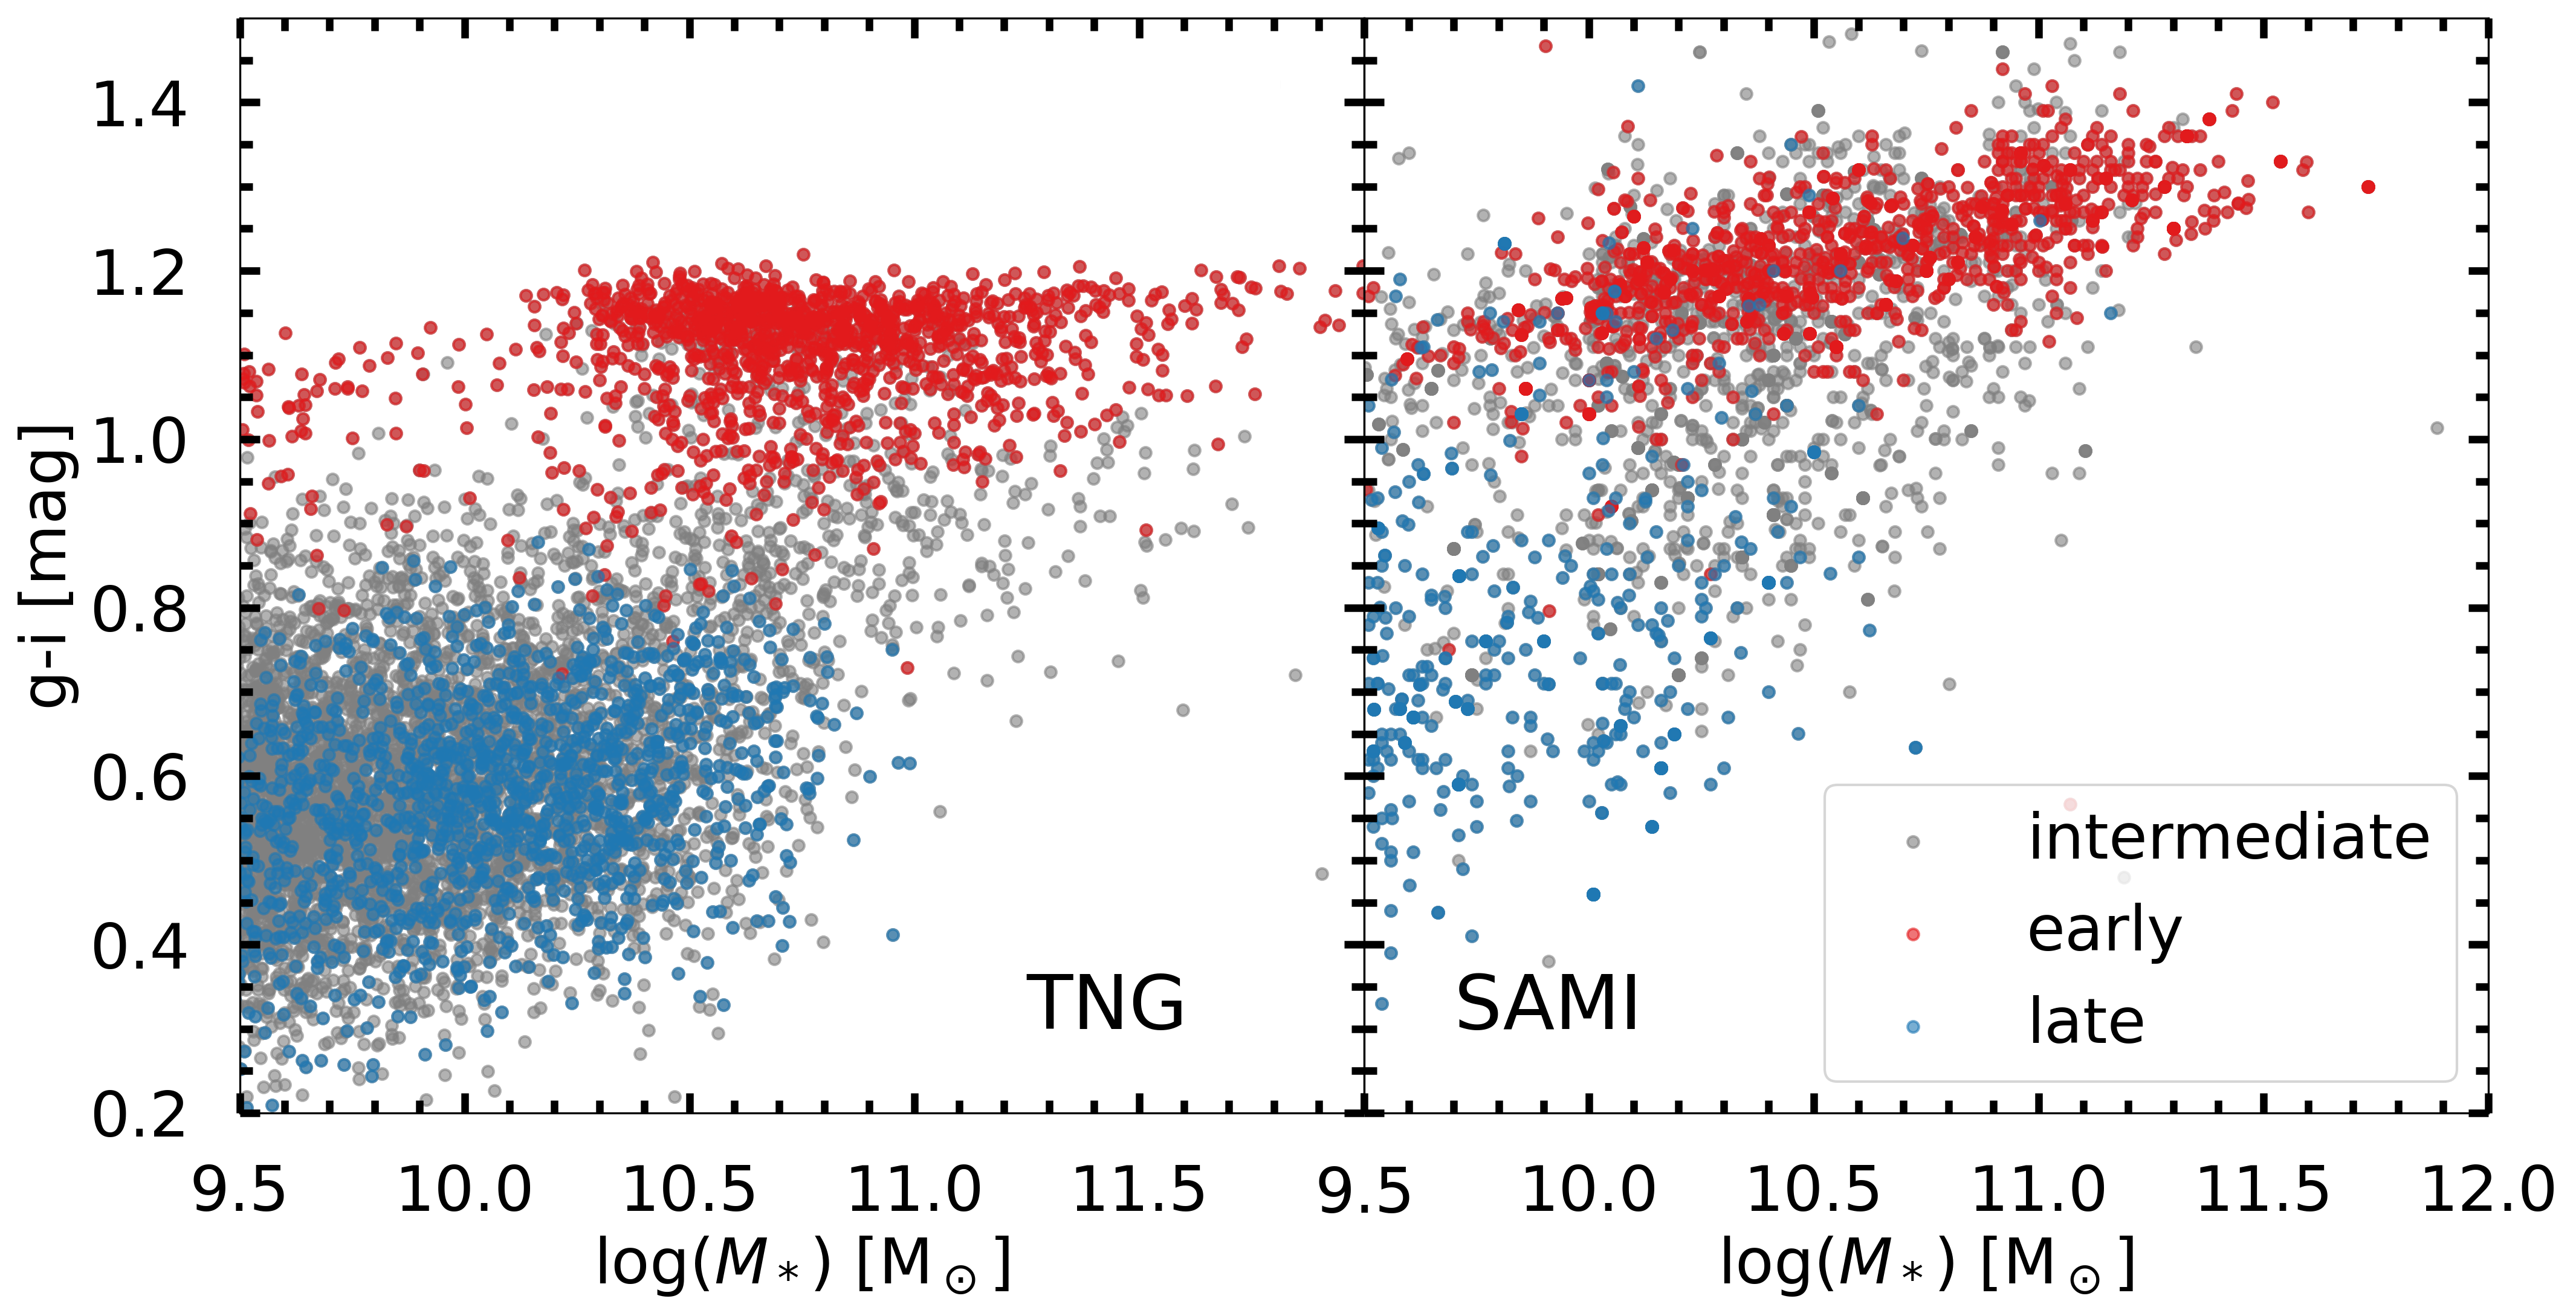
\includegraphics[width=\textwidth]{images/CB.png}
    \caption{Left: Color-mass diagram showing the TNG galaxy distribution for early type (red), late type (blue) and intermediate type (grey) galaxies. Right: Similar color-mass diagram showing the SAMI galaxy distribution.}
    \label{CB}
\end{figure}

\begin{figure}
    \centering
    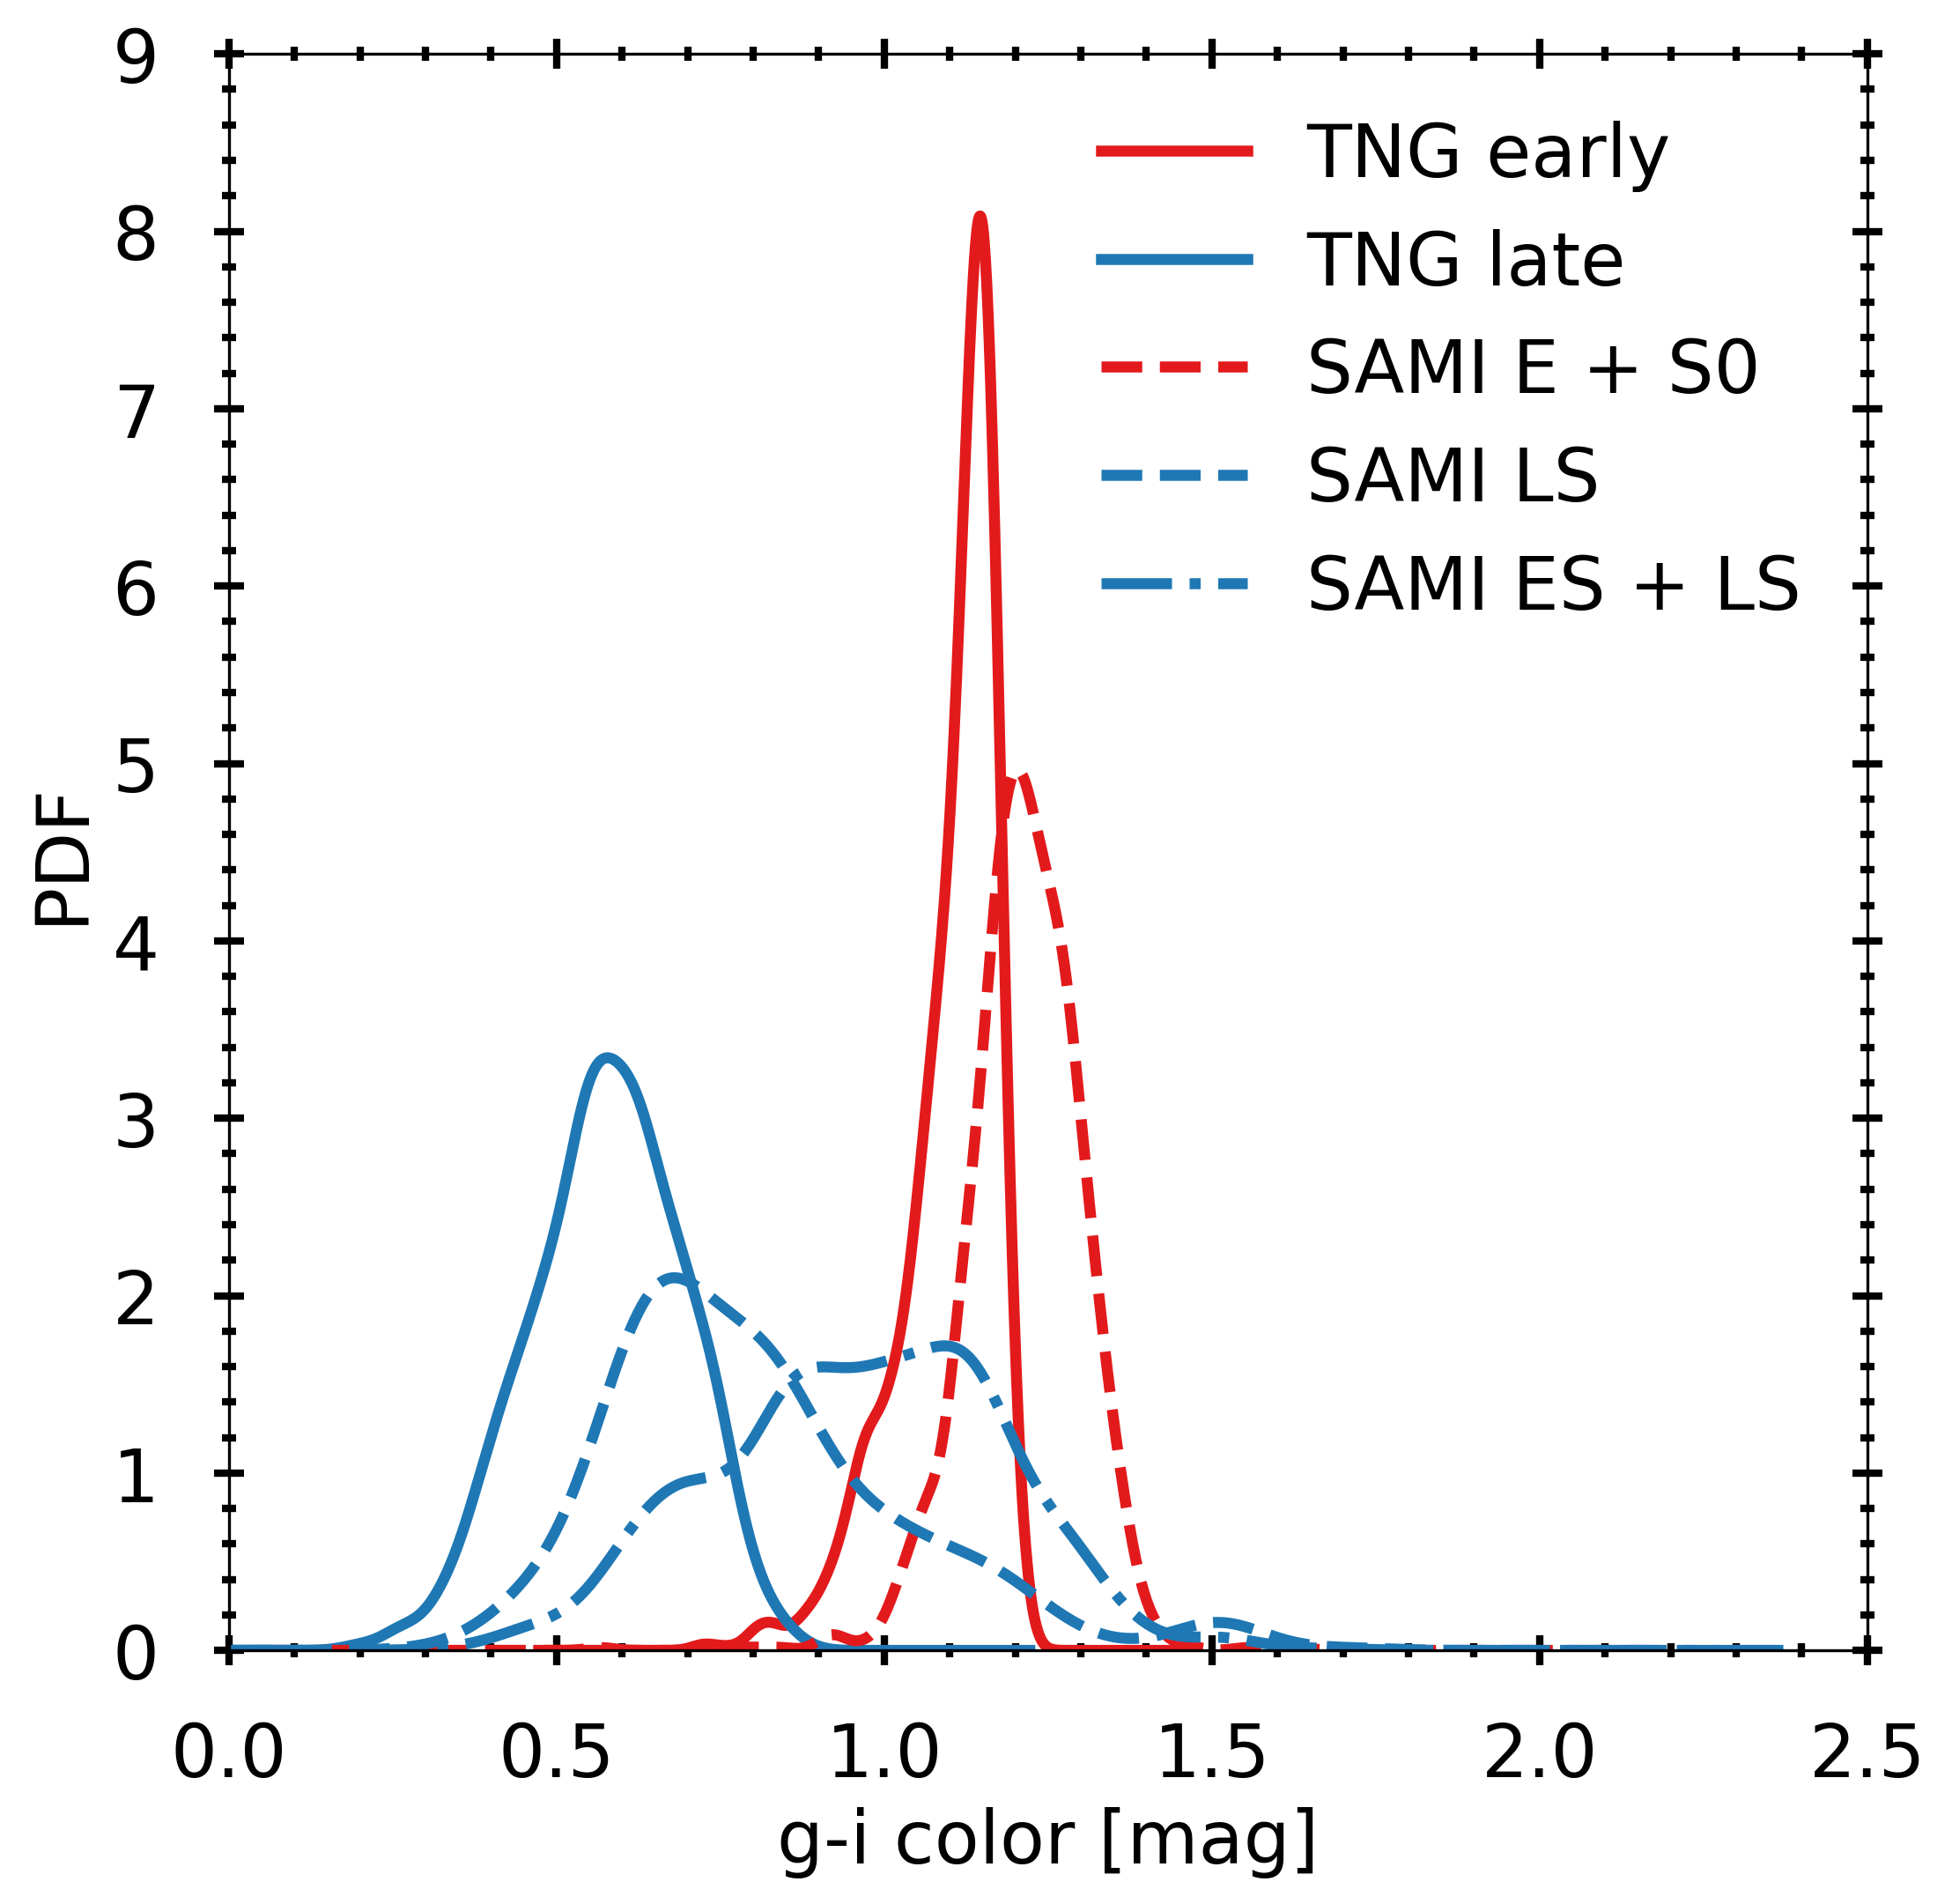
\includegraphics[width=0.9\textwidth]{images/CB_PDF.png}
    \caption{The distribution of g-i color in TNG and SAMI. Kernel density weighted PDF (with Gaussian kernels) are shown for TNG early and late types (red and blue solid lines) as well as for SAMI (red and blue dashed lines). For SAMI late type, two different morphology selections are shown. The short-dashed line show the PDF for the late spiral galaxies and the long-dashed lines show the PDf for the early and late spirals. The values are not normalized, so the height of the peak is not comparable, but the x-position and width is.}
    \label{CB_PDF}
\end{figure}

\newpage
\section{Discussions and conclusion} \label{discussions}
%summary

%what was done
In this work the IllustrisTNG TNG-100 simulation has been analysed to extract information about the statistics of galaxy properties. The properties studied are stellar mass, halo mass, half-mass radius, velocities and color. Several different methods of calculating these properties have been employed, and are compared against each other as well as against the SUBFIND group catalog. Finally the TNG results were compared against the SAMI observational data as well as some auxiliary observational results to evaluate the efficiency of TNG in reproducing galaxy properties.

\subsection{Discussion and summary}
It was found that TNG stellar mass estimates are highly dependent upon the way that the galaxy size is defined. For the largest galaxies ($M_{halo} > 10^{13.5} M_\odot$), stellar mass varies by as much as 40 \% depending on the aperture within which the mass is calculated. The reason for this is that we are ``cutting off'' the continuous stellar particle distribution in the halo at the aperture radius. For large diffuse galaxies that can extend over 100 kpc from the center of the halo, the effect will be most pronounced, and this is what we are indeed finding. A direct comparison of stellar masses found in galaxies between TNG and other studies would therefore be significantly affected by the choice of how stellar mass is defined, and this must be taken into account when doing any kind of comparison. 


The stellar-to-halo mass relation for TNG and two recent observational results, \textcite{Behroozi2019} and \textcite{Kravtsov2018} were then compared. TNG shows excellent agreement for the SHMR compared to \textcite{Behroozi2019} in the mass range $10^{9.5} M_\odot < M_\ast < 10^{11} M_\odot$. However, in the high mass range $M_{halo} > 10^{12.3} M_\odot$ TNG SHMR has a steeper slope than that found in observations. \textcite{Kravtsov2018} suggest that works like \textcite{Behroozi2019} and \textcite{Zanisi2019} underestimate the stellar mass, and their results for $M_{halo} > 10^{13} M_\odot$ halos are more similar to TNG $M^{SUBF}_\ast$. The slope of TNG is still too steep however. These results reproduce the findings in \textcite{Pillepich2017}, where also the galaxy stellar mass function is studied and compared to observational results. They show that there is an overabundance of massive galaxies in the simulations, and that galaxy stellar mass definitions have a large impact on the size of this mismatch. They also point out the intrinsic difficulty in separating the main galaxy's stellar mass from the inter-cluster light of the largest halos, and advocate that this should not be attempted. Stopping star formation in simulations is very difficult, and it requires a fine balance between allowing smaller galaxies to grow while quenching the star formation in the largest galaxies. There is therefore a good chance that TNG massive galaxies have grown too large \parencite[as suggested by][]{Vazquez2020}, but there is also a chance that observations are simply missing the low surface brightness outer parts of massive elliptical galaxies \parencite[see e.g.,][]{DSouza2015}. A suggestion to mitigate this issue is to not try to actually measure the entire galaxy, but use a stellar mass measurement within a fixed aperture in physical kiloparsecs \parencite[see e.g.,][]{Pillepich2017, Kravtsov2018}. That would be a clear definition, and should be possible to do for both observational data and simulations. This would be an interesting project for future research.


The stellar half-mass radii were then estimated using the different stellar mass definitions (based on different galaxy size assumptions). The results as shown in Figure \ref{SM_R_TNG} show a divergence in half-mass radius around $M^{SUBF}_\ast = 10^{11} M_\odot$. This is a consequence of the large difference in the stellar mass definitions. Both 3D and projected radius were calculated, and it was found that scaling the 3D radius by a factor of $3/4$ as proposed by \textcite{Wolf2010} is an excellent approximation to the average calculated projected radius. 
The size-mass relation of TNG is almost flat at masses below $10^{10.5} M_{\odot}$. This tells us that TNG galaxies become more dense as they grow in size, until they reach the characteristic stellar mass $M_\ast = 10^{10.5} M_{\odot}$, where they start to expand with increasing mass. This trend is much less profound in the observational SAMI data, which has a positive slope across the mass spectrum. It is important to note that there is a large scatter in both observation and simulation results as well as uncertainties which are not accounted for in this study. TNG galaxies in this flat regime have larger median effective radius than SAMI galaxies by about 0.1 dex (26 \%), but have a 25-75 \% spread of $\pm$ 0.1 dex. Keeping this in mind, the similarity in the stellar mass - effective radius relation between SAMI and TNG is remarkable. 

There is however a larger difference between observations and simulations when looking at early and late type galaxies separately. It was also found that this relation is sensitively dependent on the selection criteria for morphology classification, both for TNG and SAMI. The most strict criteria, which should give a ``cleaner'' sample of only very elliptical and very disky galaxies, are the ones that diverge the most when comparing observations and simulation. This is most profound when looking at the strict criteria for late type galaxies, where TNG galaxies are $\sim 0.2$ dex (58 \%) smaller for $M_\ast \sim 10^{10.5} M_\odot$ compared to SAMI.

A very important point to remember when considering these results is that they depend on the comparison between half-mass radius and half-light radius, which would be the same if the mass-to-light ratio was constant throughout the stellar mass profile of each galaxy. This does not appear to be the case, as it has been found that luminosity-weighted characteristic sizes are larger for late type galaxies \parencite{Sande2018}. They attribute this to the bulge part of a galaxy, which is redder and thus weighted less in the r-band than the bluer disk in the outer parts of the galaxies. A better comparison would then be to calculate the half-light radius for TNG galaxies. This was done in \textcite{Genel2017}, where they found that $R_{hl}$ are similar to $R_{hm}$ up to the characteristic stellar mass of $M_\ast = 10^{10.5} M_\odot$, where they converge with the 3D half-mass radius $r_{hm}$ that are significantly larger than $R_{hm}$ across all masses (see Figure \ref{SM_R_TNG}).


Rotational velocity was also studied, and has no dependency on radius beyond $2 \times r_{hm}$, as expected. The Tully-Fisher relation of TNG late-type galaxies gives similar values as observations while having a slightly shallower slope. As the late type galaxies in the TNG sample generally do not exceed $M_\ast = 10^{11} M_{\odot}$, we do not see any difference in the TFR for stellar mass definitions $M_\ast^{15r200}$ or $M_\ast^{SUBF}$ compared to $M_\ast^{30kpc}$. Using the stellar mass measurement within $2 \times r_{hm}^{SUBF}$ would decrease the slope further, making for an even worse fit to the observational data. The SAMI fit is based on a sample of galaxies that span a larger stellar mass range than the TNG galaxies studied here, from $10^{7.5} M_{\odot} - 10^{11.5} M_{\odot}$. The TFR extends across the entire mass range though, with a higher scatter at low stellar masses, so it is still comparable to the TNG data which only spans a range of about $10^{9.5} M_{\odot} - 10^{11} M_{\odot}$. 


Next, the different particle's contribution to the total velocity dispersion in the subhalos was looked at, showing that gas particles have significantly lower velocities than stars and dark matter. The dark matter velocity dispersion is similar for the entire mass range of subhalos, while the stellar velocity dispersion was lower for both the smallest and the largest galaxies, with a maximum for galaxies with stellar mass $10^{10.5} M_\odot$. The stellar velocity dispersion has little dependency on galaxy aperture size down to $r^{SUBF}_{hm}$, and projection effects are minimal. TNG galaxies have a similar slope in the Faber-Jackson relation compared to observations, but have a lower zero point by about 0.1 dex.  From this, it would seem that velocity dispersions in TNG are lower than those seen in observations at redshift $z=0$. Based on the above analysis, it does not seem like this can be attributed to projection effects or the size of the volume within which the velocity dispersion is calculated, but rather the velocities of the simulated stellar particles are in general lower than that which is observed in the stars of real elliptical galaxies. This is in agreement with the results of \textcite{Sande2018}, as they find simulated velocity dispersions to be lower than in observations. 


Finally, TNG produces a distinctly bimodal galaxy color distribution in the g-i color, as already determined by \textcite{Nelson2017}. The color distribution of the subhalos was not affected by any of the studied aperture sizes. Bimodality matches well with galaxy morphology classification, even with the least strict criteria where only sSFR was considered. Compared to SAMI observations the color distribution may be too binary as the gradual increase in redness with increasing stellar mass which is found in the observations is missing in the simulation data. This is also mentioned by \textcite{Nelson2017}, who interestingly suggests that this is due to their choice of a 30 kpc aperture which excludes parts of the larger galaxies. This turns out to not be the case as mentioned earlier. Their other suggested solution was that there is a discrepancy in the relatively simple TNG dust modeling, which then seems to be plausible. TNG galaxies are also slightly bluer than the SAMI galaxies, reflecting the missing reddening with stellar mass within the two galaxy populations. It was also found that TNG early and late type galaxies kept their color bimodality regardless of morphology selection criteria, while SAMI late type galaxies changed significantly when using the less strict criteria of late type galaxies by including so-called ``early spirals'' in the sample. This furthers the importance of paying attention to the galaxy classification methods.


To summarise, the main findings are as follows.
%Conclusions bullet points
\begin{itemize}
	\item Of the properties studied here, the SUBFIND values are great to use for rotational velocity and color. The SUBFIND velocity dispersion measurement should not be used as a proxy for gas velocity dispersion, and is not a very precise estimate for stellar velocity dispersion either. SUBFIND values should be used with caution for stellar mass and half-mass radius for halos with a total mass larger than $10^{13} M_\odot$.
	\item Projected half-mass radii can be calculated using the excellent approximate relation $R_{e} \approx 3/4 \times r_{e}$. Projection effects on velocity dispersion measurements for early type galaxies are neglible.
	\item Galaxy stellar mass is heavily dependent on aperture size in both simulations and observations for stellar masses above $10^{11} M_\odot$. When comparing the two, it is beneficial to use the same definition of stellar mass.
	\item Galaxy morphology classification should be treated carefully when comparing sizes and color. Specifically it was found that using a ``strict'' classification method (using both specific star formation rate and rotational-to-kinetic energy ratio for TNG galaxies and only the most elliptical and most late type spirals for SAMI) gave better agreement in the color bimodality, but a worse agreement in the size-mass relation compared to a ``less strict'' method (using only specific star formation rate for TNG galaxies and including a broader range of early and late types in SAMI).
	\item Comparing TNG scaling relations to observations, the TNG SHMR slope is similar to observations for halo masses up to $10^{12.3} M_\odot$ where it becomes steeper. The size-mass relation shows excellent agreement for the entire galaxy population, but shows differences when separated into early and late type galaxies. The TFR of TNG has a shallower slope than observations, but values fall within the uncertainties. The FJ relation of TNG and observations has a similar slope, but TNG has a slightly lower zero-point. The color bimodality in TNG is in good agreement with observations, although the slope in the relation seems too flat. All in all, the scaling relations of TNG exhibit the expected trends found in observational data, despite some discrepancies which do not seem to be related to the way in which the properties are calculated.
	

\end{itemize}

\subsection{Reflection and way forward}
The newest set of hydrodynamical cosmological simulations like TNG are so good at recreating the structures and properties of the Universe at cosmological scales that comparisons against observations are becoming more and more relevant and useful. This also means that observational and numerical astrophysicists must become even better at doing these kinds of comparisons in a fair and meaningful way. Efforts are being made in this direction, and especially \textcite{Sande2018} stands out as going to great lengths in reproducing the observational methods of calculating size and kinematic properties for the three different simulations they study. They do not however mention much about stellar mass measurements, and so a study similar to this on several other properties like stellar mass and color would be a great contribution towards this goal.

%reflection and way forward
Explicitly stating all definitions and methods used in a scientific work is extremely important for it to be relevant in the greater scope of astrophysics research. As cosmological simulations essentially are ``black boxes'' to outside users, the way that the data is post-processed and interpreted is non-trivial in every sense, especially when comparing against observational data. Standards are quite different in the observational and numerical sections of astrophysics, so it can be hard to make meaningful comparisons (especially as someone new to the field). Developing a standard method of calculating properties and comparing them would be a step in the direction of making it easier to navigate the increasingly large amount of research done in the field of galaxy formation and evolution. In this age of digital revolution, huge amounts of data are acquired each year, both from the development of better observational instruments, creating new ways of analysing old data and from numerical experiments like IllustrisTNG. This means that new research is constantly being published, and it is hard to keep up with the inflow of information. That only makes it even more important to make sure that our works are easily reproducible and that all methods and definitions are unambiguously defined, preferably accompanied by a reflection on the impact of those choices. This will lead to more clarity, and eventually to a much more comparable set of works published in the future.

%\section{Conclusions} \label{conclusions}
%\input{sections/conclusions}

\medskip
\printbibliography
%\bibliographystyle{aa}
%\bibliography{mybib} % if your bibtex file is called example.bib
\end{document}
